\chapter{Implementasi dan Pengujian}
\label{chap:implementasipengujian}

\section{Implementasi}
\label{sec:implementasi}

\subsection{Lingkungan Implementasi}
\label{sec:lingkunganimplementasi}
Impelementasi dilakukan dengan menggunakan laptop peneliti. Berikut adalah spesifikasi laptop peneliti:
\begin{enumerate}
	\item Processor: Intel(R) Core(TM)2 Duo 2.40 GHz
	\item RAM: 2048 MB
	\item Sistem Operasi: Windows 7 Ultimate 32-bit (6.1, Build 7601)
	\item Versi Java: 1.8.0\_91
	\item Versi Play Framework: 2.4.3
	\item Browser: Google Chrome 50.0.2661.94
\end{enumerate}

\subsection{Hasil Implementasi}
\label{sec:hasilimplementasi}
Hasil implementasi dari penelitian ini adalah aplikasi berbasis \textit{web} yang menggunakan Play Framework. Aplikasi dapat diakses ke jaringan lokal milik peneliti melalui URL \url{http://localhost/bukitjarian/}. Aplikasi KIRI \textit{Dashboard} terbagi ke dalam 16 bagian.
\begin{enumerate}
	\item \textbf{Bagian \textit{Register}}\\
	Bagian ini merupakan bagian untuk mendaftarkan pengguna baru ke dalam sistem KIRI. Pengguna dapat mengisi alamat \textit{email}, nama lengkap, dan nama perusahaan pada formulir registrasi (Gambar \ref{fig:5_register_1}). Jika pendaftaran berhasil (Gambar \ref{fig:5_register_2}), pengguna dapat langsung mengecek kotak masuk \textit{email} yang didaftarkan (Gambar \ref{fig:5_register_3}).

	\begin{figure}[htbp]
		\centering
			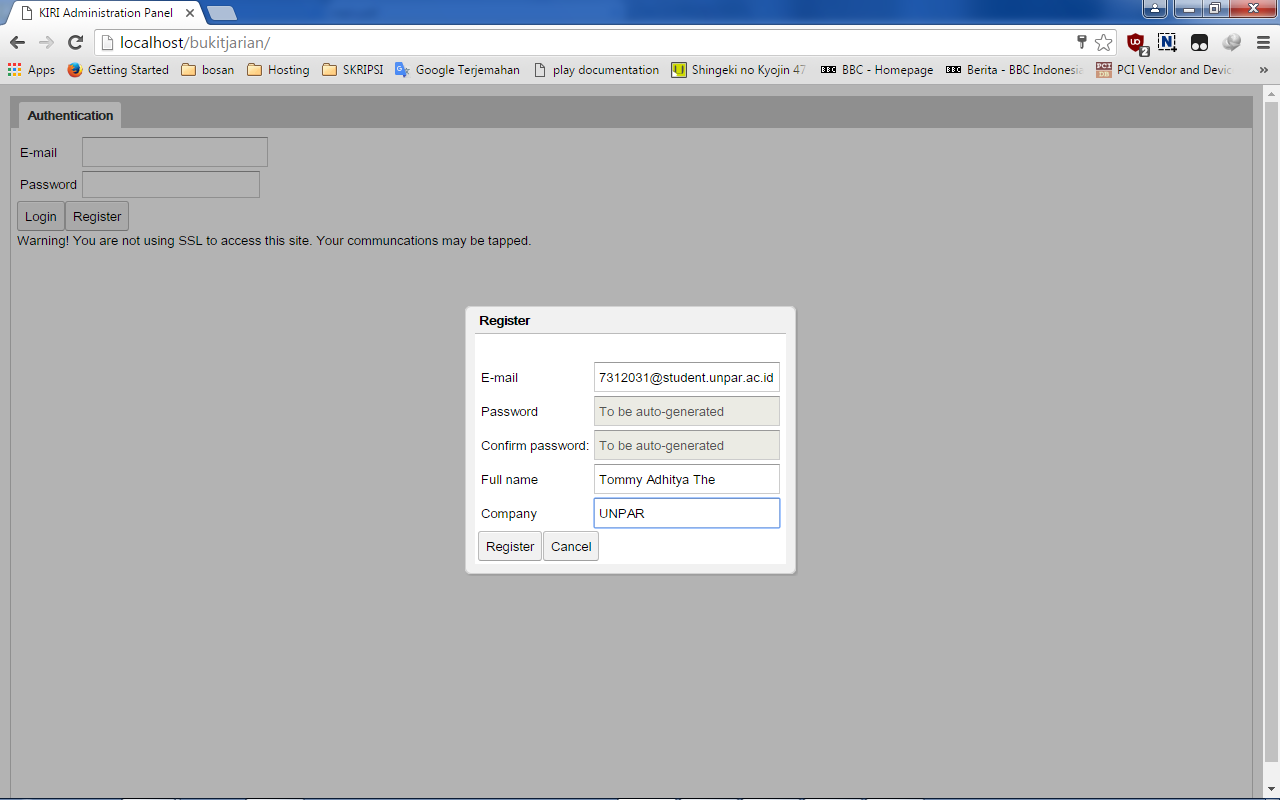
\includegraphics[scale=0.45]{Gambar/5_register_1.png}
		\caption{Formulir registrasi}
		\label{fig:5_register_1}
	\end{figure}

	\begin{figure}[htbp]
		\centering
			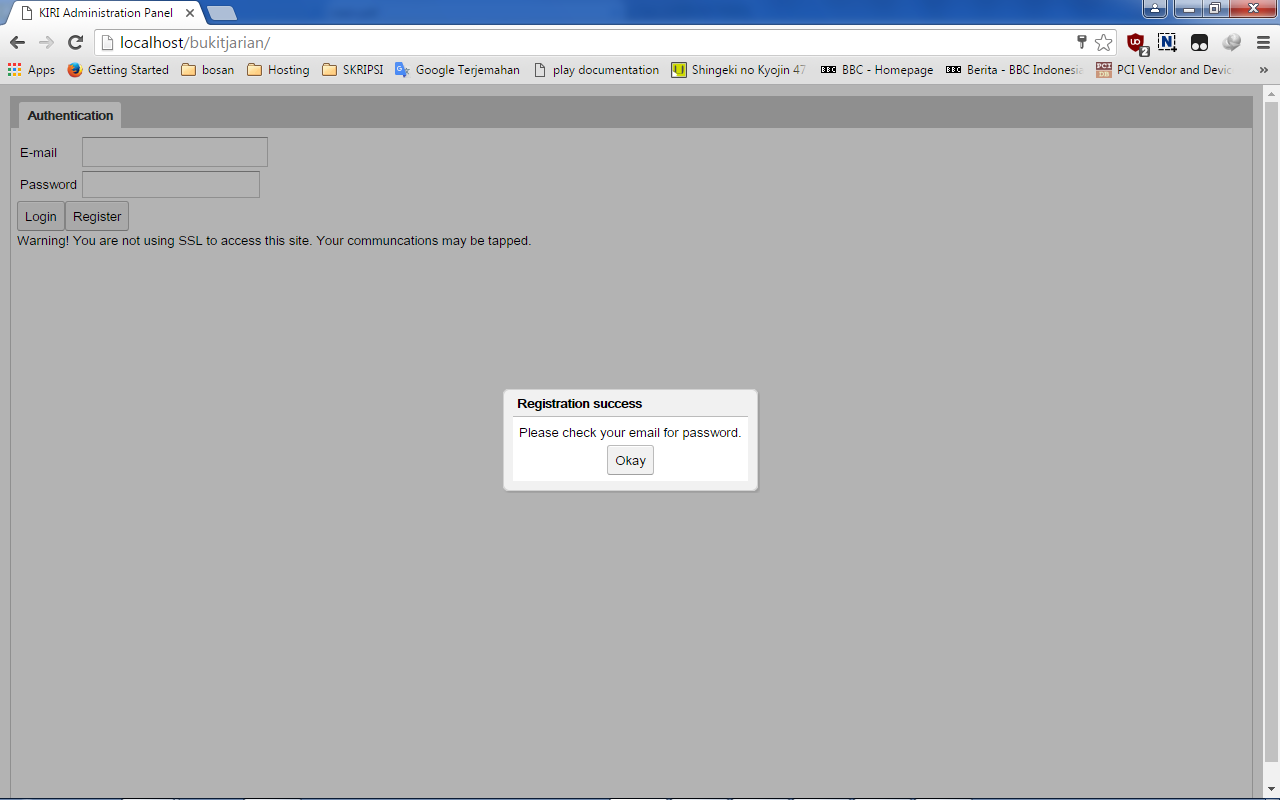
\includegraphics[scale=0.45]{Gambar/5_register_2.png}
		\caption{Registrasi berhasil}
		\label{fig:5_register_2}
	\end{figure}

	\begin{figure}[htbp]
		\centering
			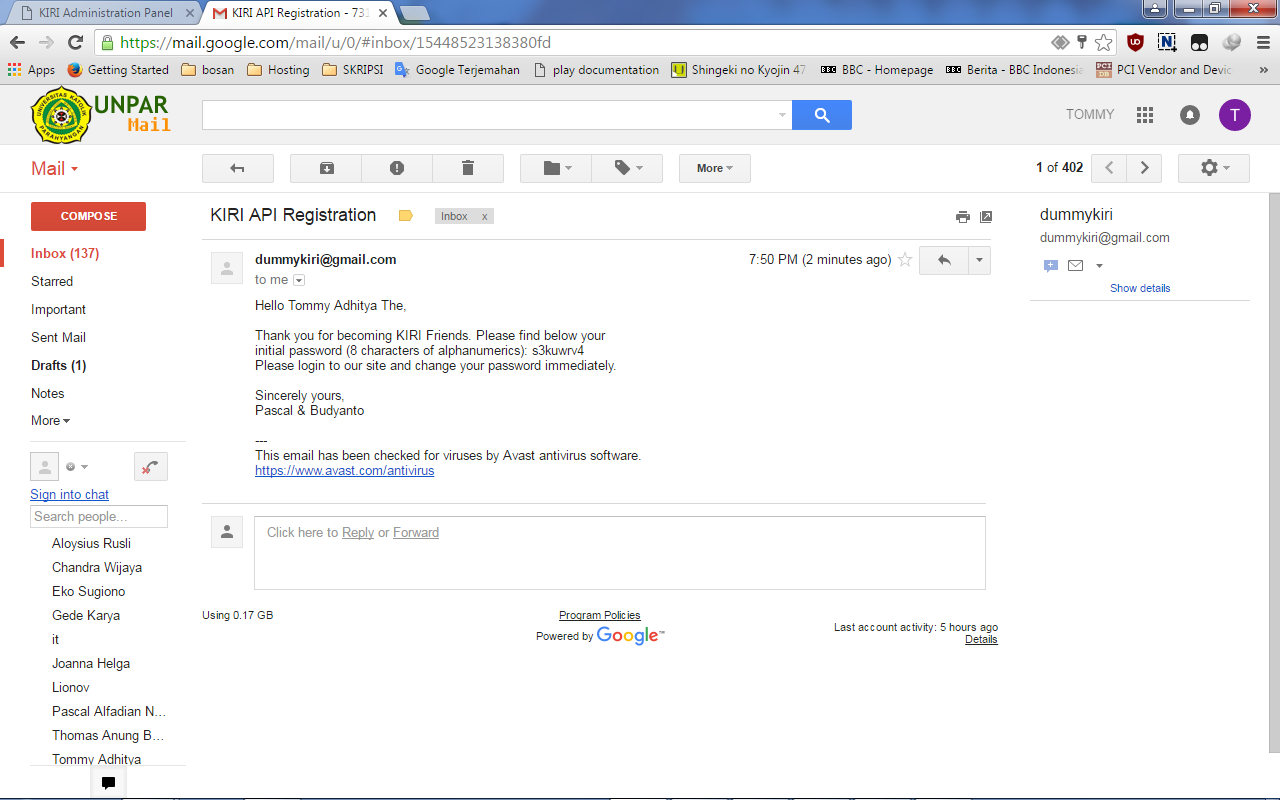
\includegraphics[scale=0.45]{Gambar/5_register_3.png}
		\caption{Kotak masuk \textit{email} pengguna}
		\label{fig:5_register_3}
	\end{figure}

	\item \textbf{Bagian \textit{Login}}\\
	Bagian ini merupakan bagian untuk masuk ke dalam sistem KIRI \textit{Dashboard} sebagai pengguna yang terdaftar. Jika \textit{email} pengguna terdaftar dan sandi yang pengguna masukkan sesuai, maka pengguna akan mendapatkan akses masuk KIRI \textit{Dashboard} (Gambar \ref{fig:5_login}).

	\begin{figure}[htbp]
		\centering
			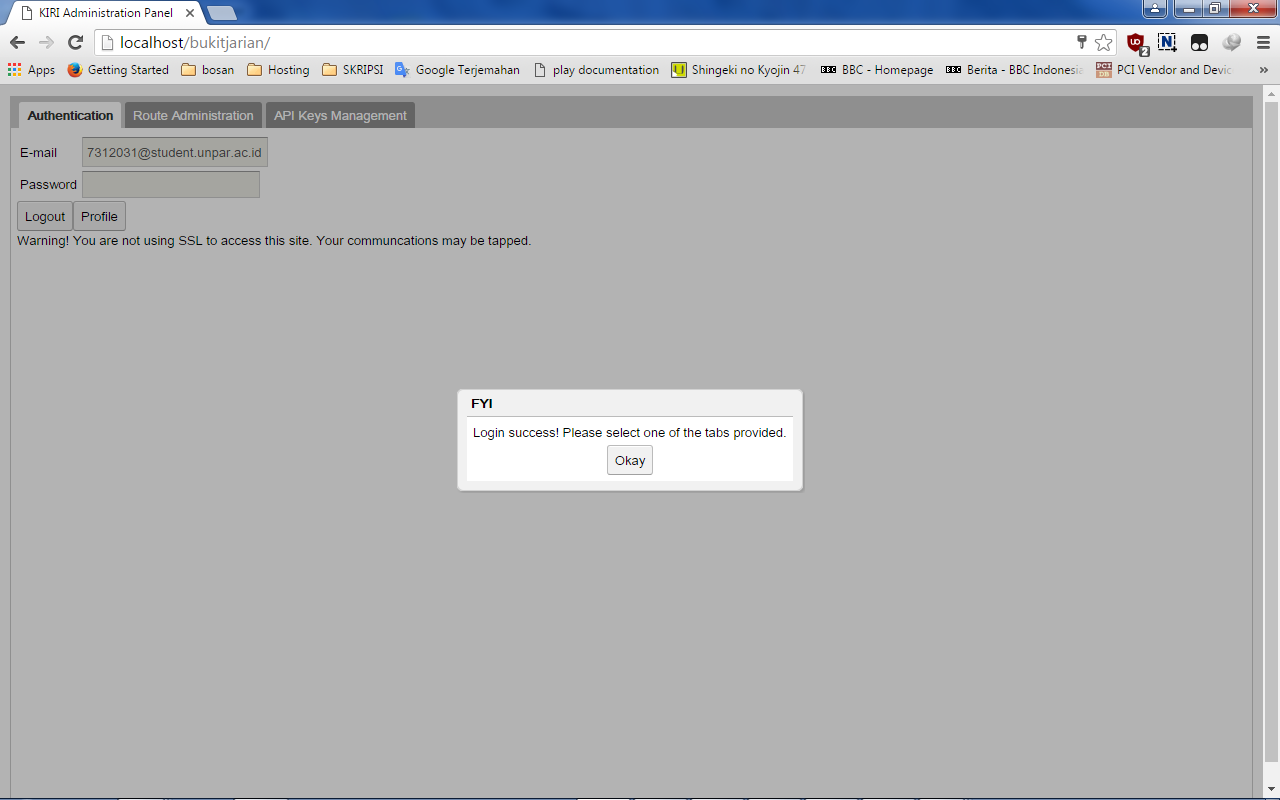
\includegraphics[scale=0.45]{Gambar/5_login.png}
		\caption{\textit{Login} dengan \textit{email} pengguna}
		\label{fig:5_login}
	\end{figure}

	\item \textbf{Bagian Pemeriksaan \textit{Login}}\\
	Bagian ini merupakan bagian pemberi hak akses rute dan API \textit{keys} kepada pengguna. Jika \textit{email} pengguna yang terdaftar memiliki hak akses terhadap rute dan API \textit{keys}, maka tampilan pengelola rute dan pengelola API \textit{keys} akan ditampilkan di layar (Gambar \ref{fig:5_login}).
	
	\item \textbf{Bagian Melihat Data Pribadi Pengguna}\\
	Bagian ini merupakan bagian yang akan menampilkan data pribadi pengguna. Data pribadi yang ditampilkan adalah nama lengkap dan nama perusahaan pengguna (Gambar \ref{fig:5_getprofil}).

	\begin{figure}[htbp]
		\centering
			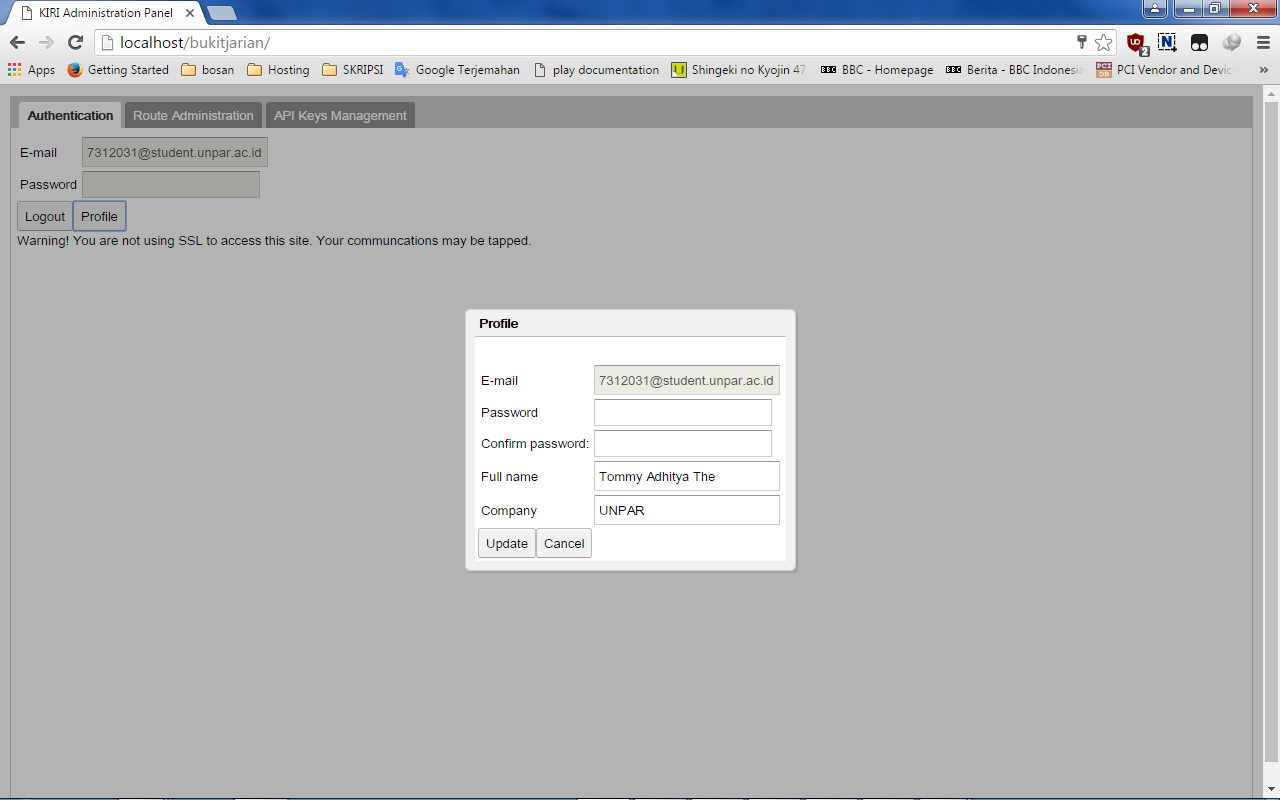
\includegraphics[scale=0.45]{Gambar/5_getprofil.png}
		\caption{Melihat data pribadi pengguna}
		\label{fig:5_getprofil}
	\end{figure}

	\item \textbf{Bagian Mengubah Data Pribadi Pengguna}\\
	Bagian ini merupakan bagian untuk mengubah data pribadi pengguna. Pengguna mengisi formulir untuk nama lengkap, nama perusahaan, dan sandi (Gambar \ref{fig:5_updateprofile_1}). Jika formulir memenuhi persyaratan sistem, maka akan muncul pesan keberhasilan (Gambar \ref{fig:5_updateprofile_2}).

	\begin{figure}[htbp]
		\centering
			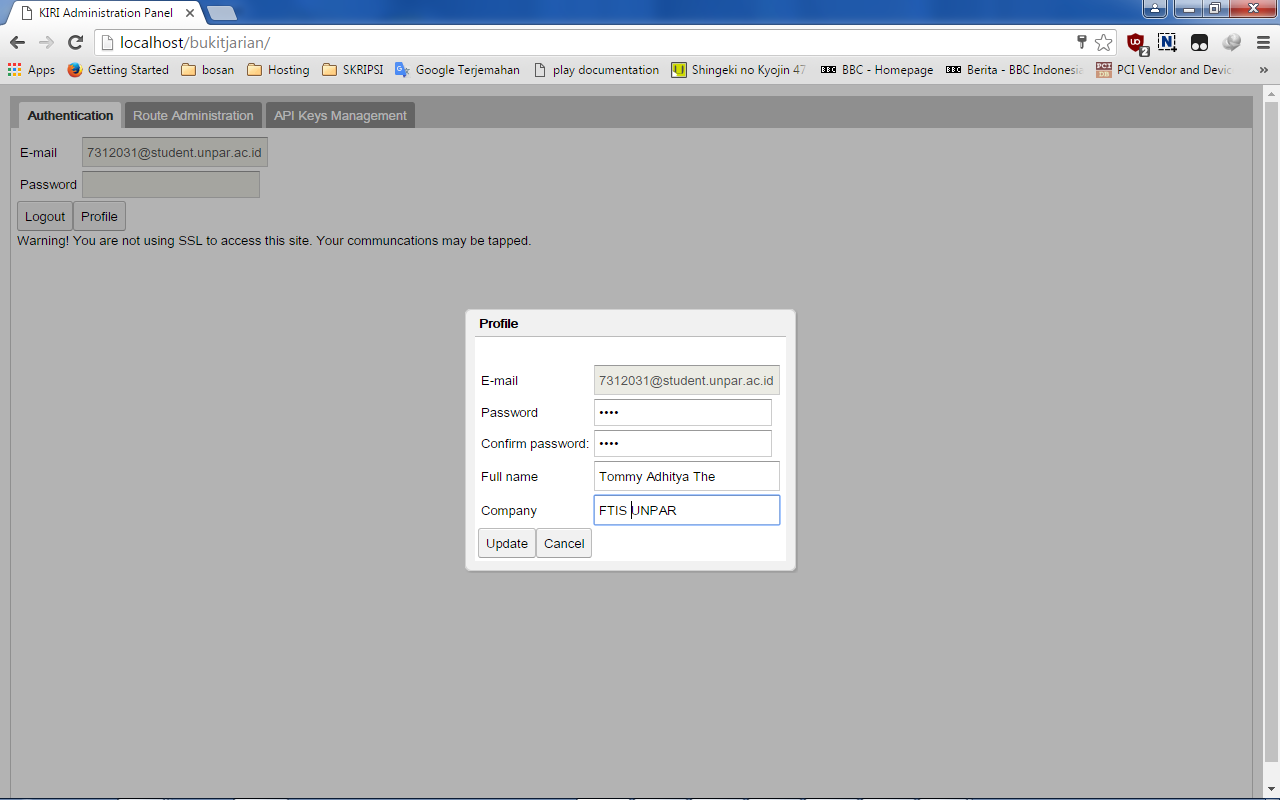
\includegraphics[scale=0.45]{Gambar/5_updateprofile_1.png}
		\caption{Formulir ubah data pribadi pengguna}
		\label{fig:5_updateprofile_1}
	\end{figure}

	\begin{figure}[htbp]
		\centering
			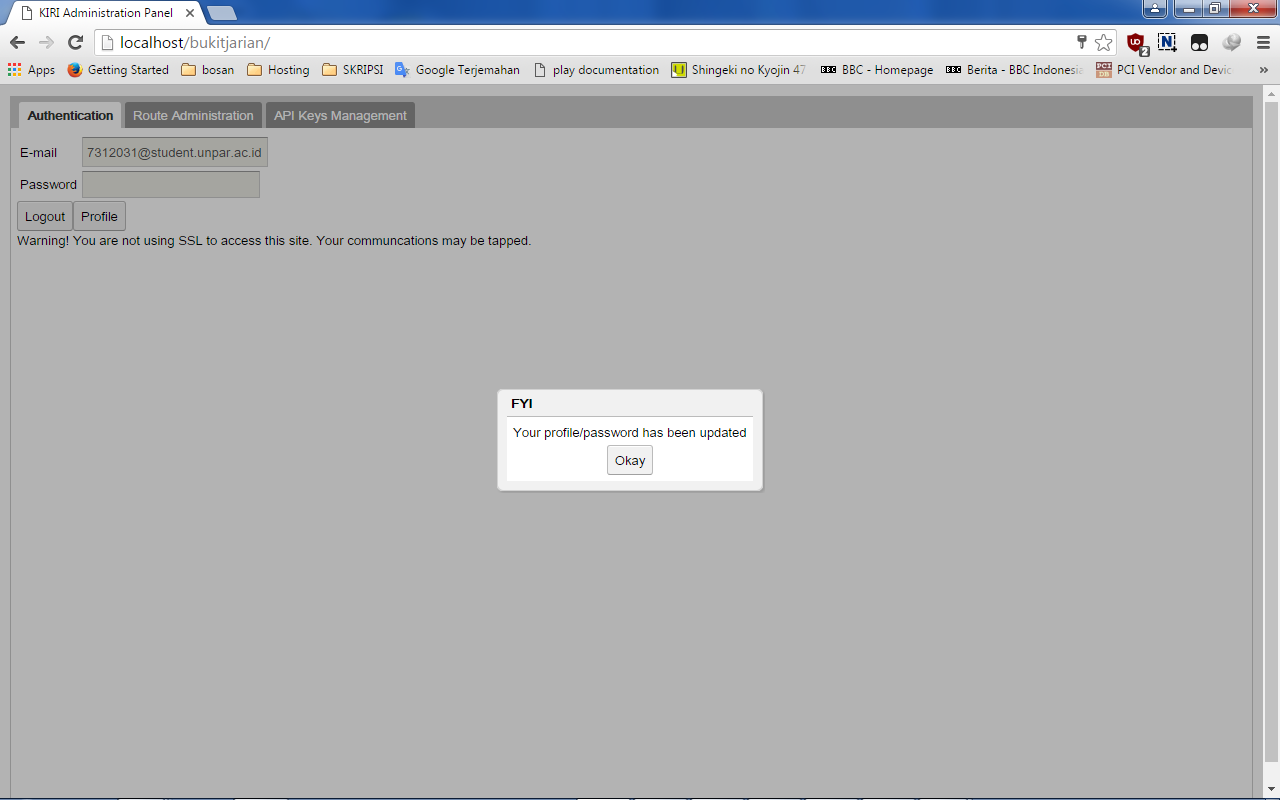
\includegraphics[scale=0.45]{Gambar/5_updateprofile_2.png}
		\caption{Ubah data pribadi pengguna berhasil}
		\label{fig:5_updateprofile_2}
	\end{figure}

	\item \textbf{Bagian Melihat Daftar API \textit{Keys}}\\
	Bagian ini merupakan bagian yang akan menampilkan daftar API \textit{keys} yang dimiliki oleh pengguna. Pengguna yang baru mendaftarkan diri belum memiliki API \textit{key} (Gambar \ref{fig:5_apikey}).

	\begin{figure}[htbp]
		\centering
			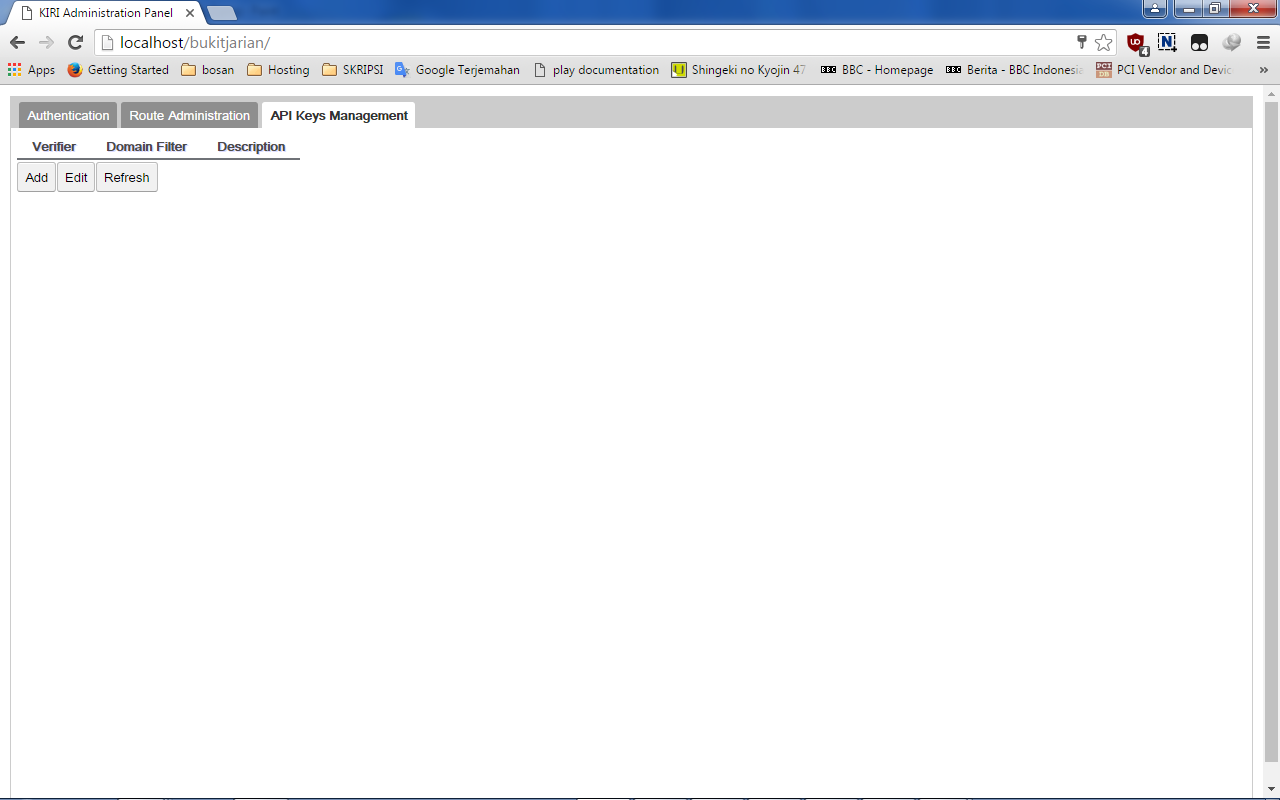
\includegraphics[scale=0.45]{Gambar/5_apikey.png}
		\caption{Daftar API \textit{keys} pengguna}
		\label{fig:5_apikey}
	\end{figure}

	\item \textbf{Bagian Menambahkan API \textit{Key}}\\
	Bagian ini merupakan bagian untuk menambahkan sebuah API \textit{key} ke dalam daftar milik pengguna. Pengguna mengisi formulir untuk nama \textit{domain} dan deskripsi mengenai API \textit{key} yang ingin ditambahkan (Gambar \ref{fig:5_addapikey_1}). Sistem KIRI akan membangun sebuah API \textit{key} baru secara acak (Gambar \ref{fig:5_addapikey_2}).

	\begin{figure}[htbp]
		\centering
			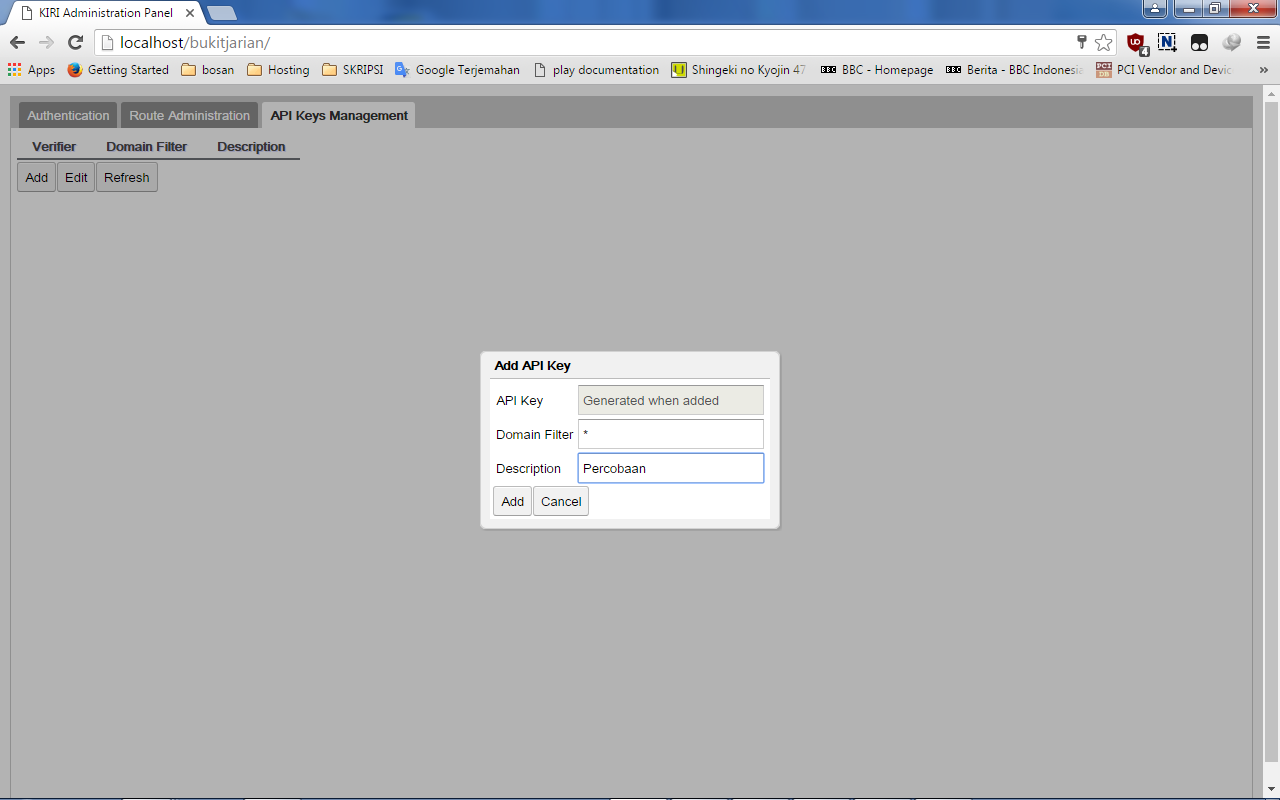
\includegraphics[scale=0.45]{Gambar/5_addapikey_1.png}
		\caption{Formulir untuk menambahkan API \textit{key}}
		\label{fig:5_addapikey_1}
	\end{figure}

	\begin{figure}[htbp]
		\centering
			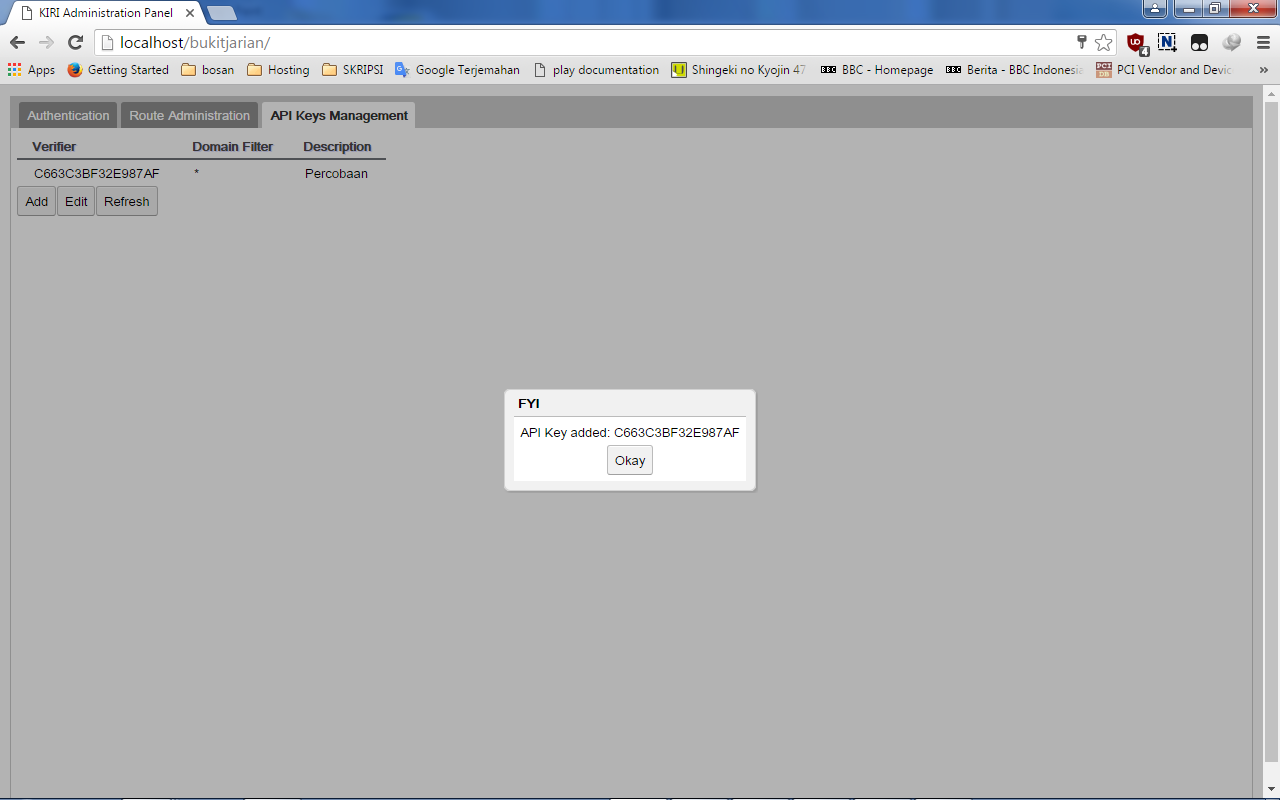
\includegraphics[scale=0.45]{Gambar/5_addapikey_2.png}
		\caption{API \textit{key} berhasil ditambahkan} 
		\label{fig:5_addapikey_2}
	\end{figure}

	\item \textbf{Bagian Mengubah API \textit{Key}}\\
	Bagian ini merupakan bagian untuk mengubah sebuah data API \textit{key} milik pengguna. Pengguna mengisi formulir untuk nama \textit{domain} dan deskripsi mengenai API \textit{key} yang ingin diubah (Gambar \ref{fig:5_editapikey_1}). Jika formulir memenuhi persyaratan sistem, maka akan muncul pesan keberhasilan (Gambar \ref{fig:5_editapikey_2}).

	\begin{figure}[htbp]
		\centering
			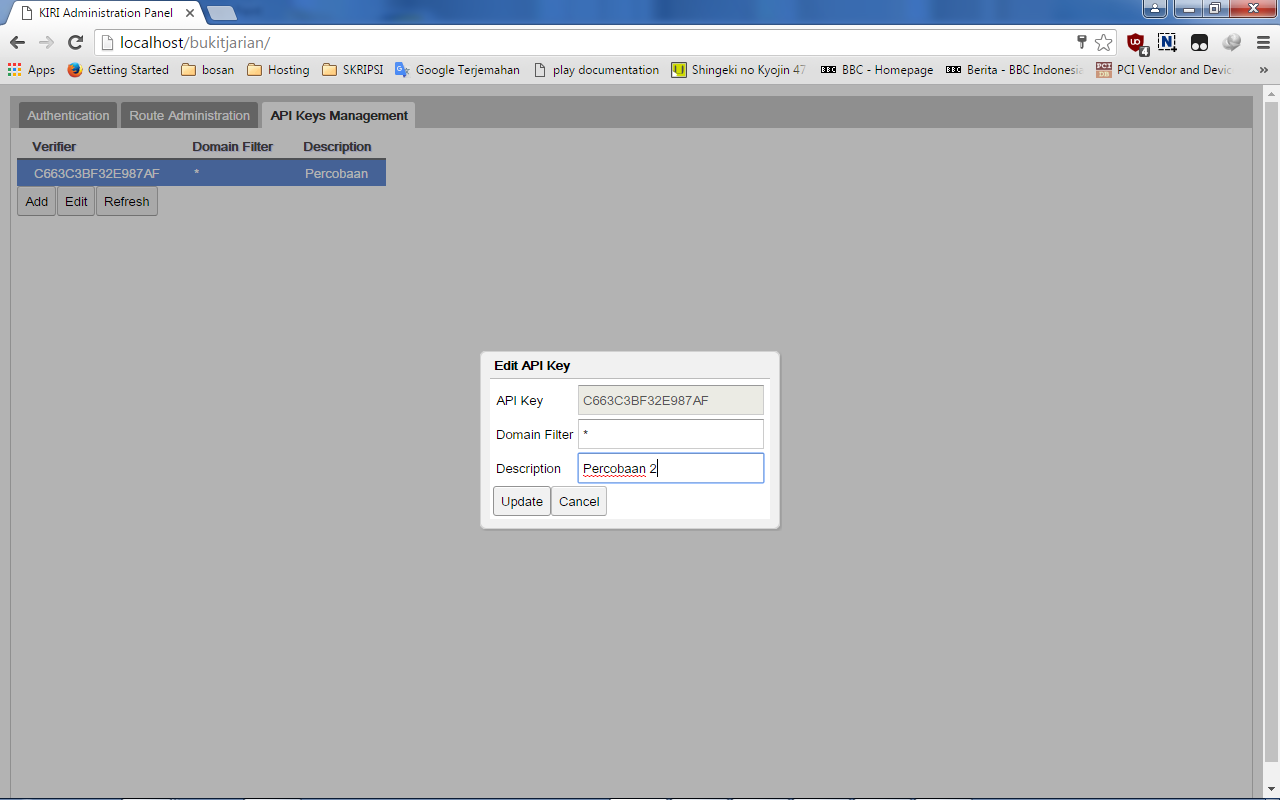
\includegraphics[scale=0.45]{Gambar/5_editapikey_1.png}
		\caption{Formulir untuk mengubah API \textit{key}}
		\label{fig:5_editapikey_1}
	\end{figure}

	\begin{figure}[htbp]
		\centering
			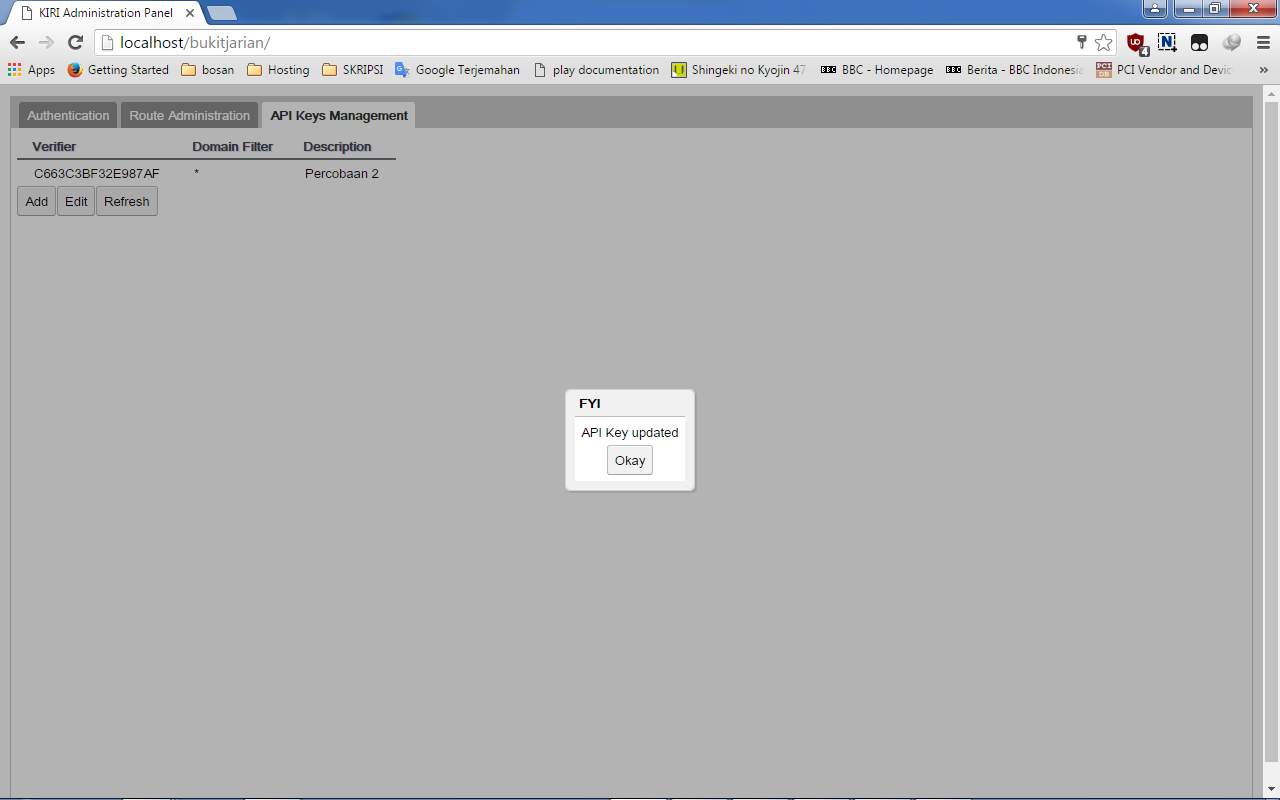
\includegraphics[scale=0.45]{Gambar/5_editapikey_2.png}
		\caption{Ubah data API \textit{key} berhasil} 
		\label{fig:5_editapikey_2}
	\end{figure}

	\item \textbf{Bagian Melihat Daftar Rute}\\
	Bagian ini merupakan bagian yang akan menampilkan daftar rute angkutan umum yang dimiliki oleh sistem KIRI (Gambar \ref{fig:5_gettracks}).

	\begin{figure}[htbp]
		\centering
			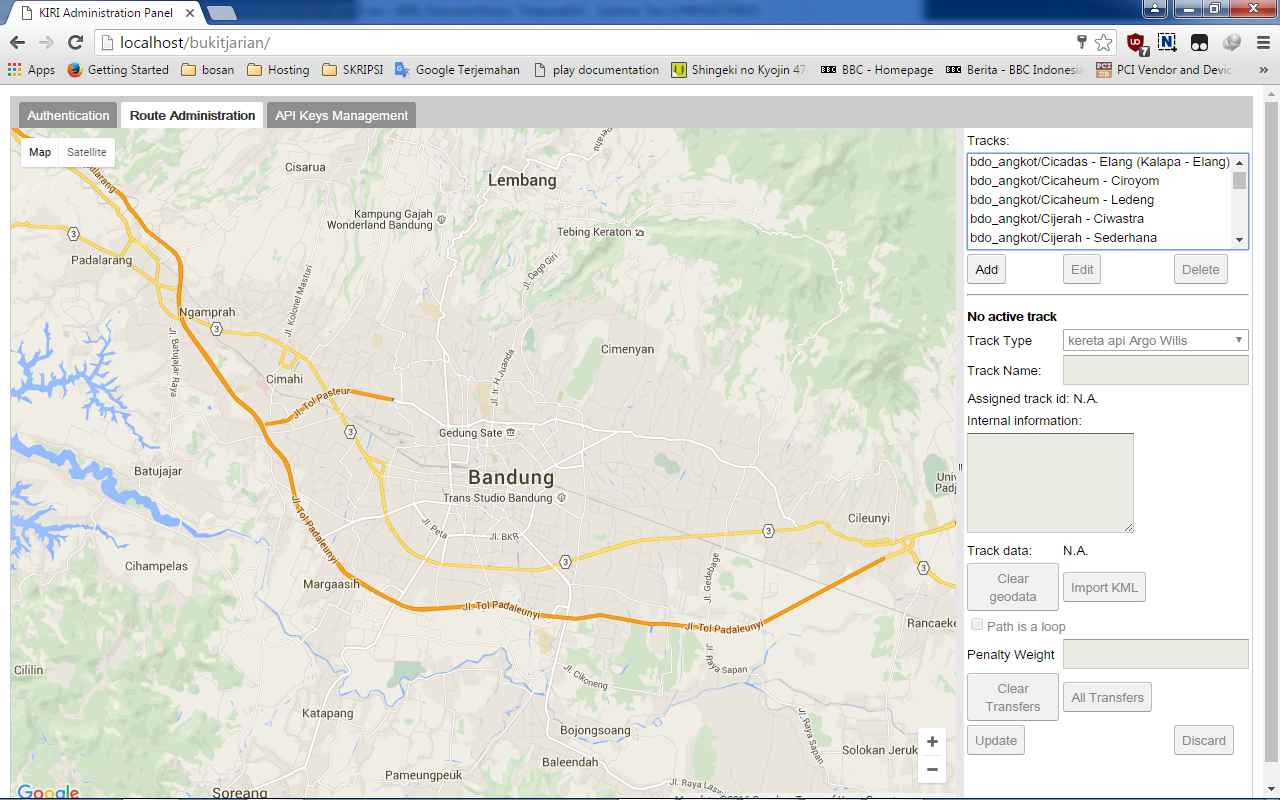
\includegraphics[scale=0.45]{Gambar/5_gettracks.png}
		\caption{Daftar rute angkutan umum sistem KIRI} 
		\label{fig:5_gettracks}
	\end{figure}

	\item \textbf{Bagian Melihat Informasi Rute secara Detail}\\
	Bagian ini merupakan bagian yang akan menampilkan detail data sebuah rute angkutan umum. Data yang ditampilkan adalah tipe angkutan umum, nama rute, informasi tambahan, data geografis dalam bentuk peta, informasi \textit{loop}, dan bobot pengali (Gambar \ref{fig:5_getdetailtrack}).

	\begin{figure}[htbp]
		\centering
			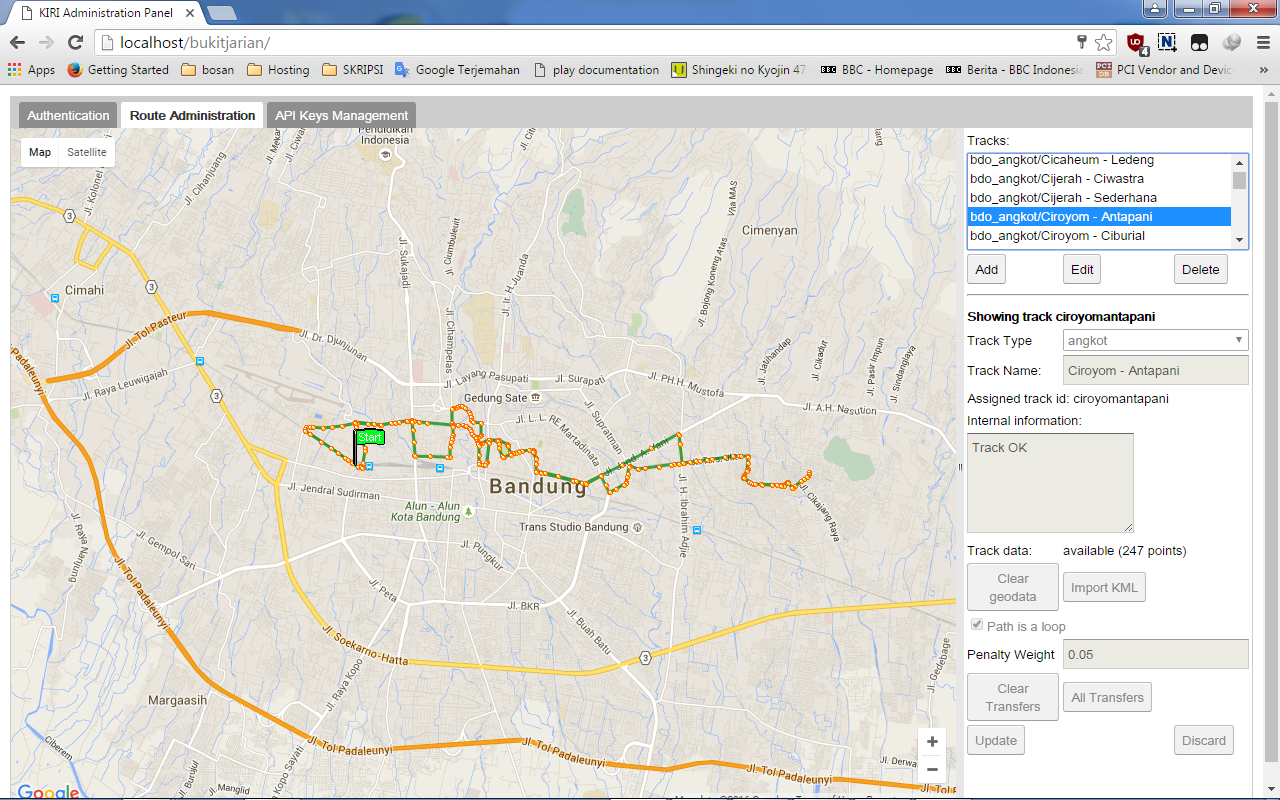
\includegraphics[scale=0.45]{Gambar/5_getdetailtrack.png}
		\caption{Detail rute angkutan umum Ciroyom-Antapani} 
		\label{fig:5_getdetailtrack}
	\end{figure}

	\item \textbf{Bagian Menambahkan Rute}\\
	Bagian ini merupakan bagian untuk menambahkan sebuah rute angkutan umum baru. Pengguna mengisi formulir untuk nama rute, informasi tambahan, bobot pengali rute, dan memilih jenis angkutan umum yang ingin ditambahkan (Gambar \ref{fig:5_addtrack_1}). Jika formulir memenuhi persyaratan sistem, maka akan rute baru akan muncul ke dalam daftar rute angkutan umum (Gambar \ref{fig:5_addtrack_2}).

	\begin{figure}[htbp]
		\centering
			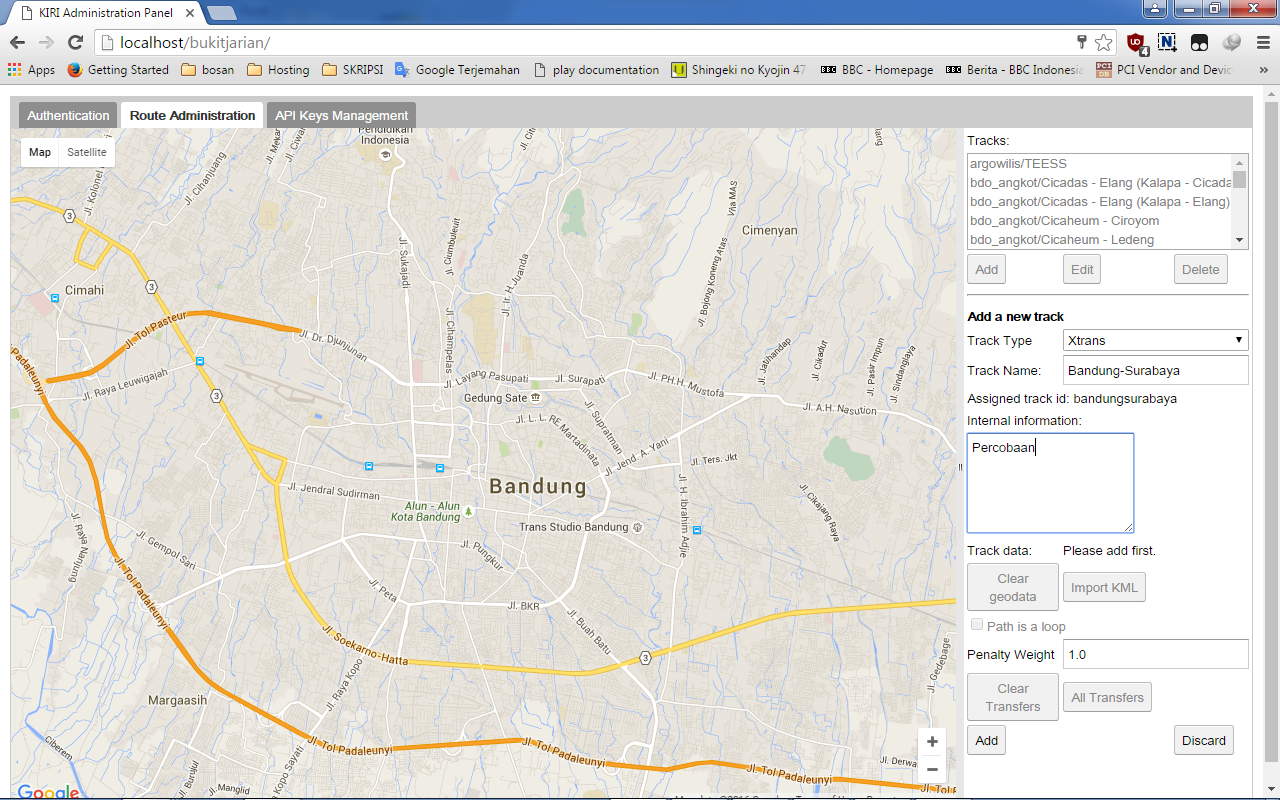
\includegraphics[scale=0.45]{Gambar/5_addtrack_1.png}
		\caption{Formulir penambahan rute angkutan umum} 
		\label{fig:5_addtrack_1}
	\end{figure}

	\begin{figure}[htbp]
		\centering
			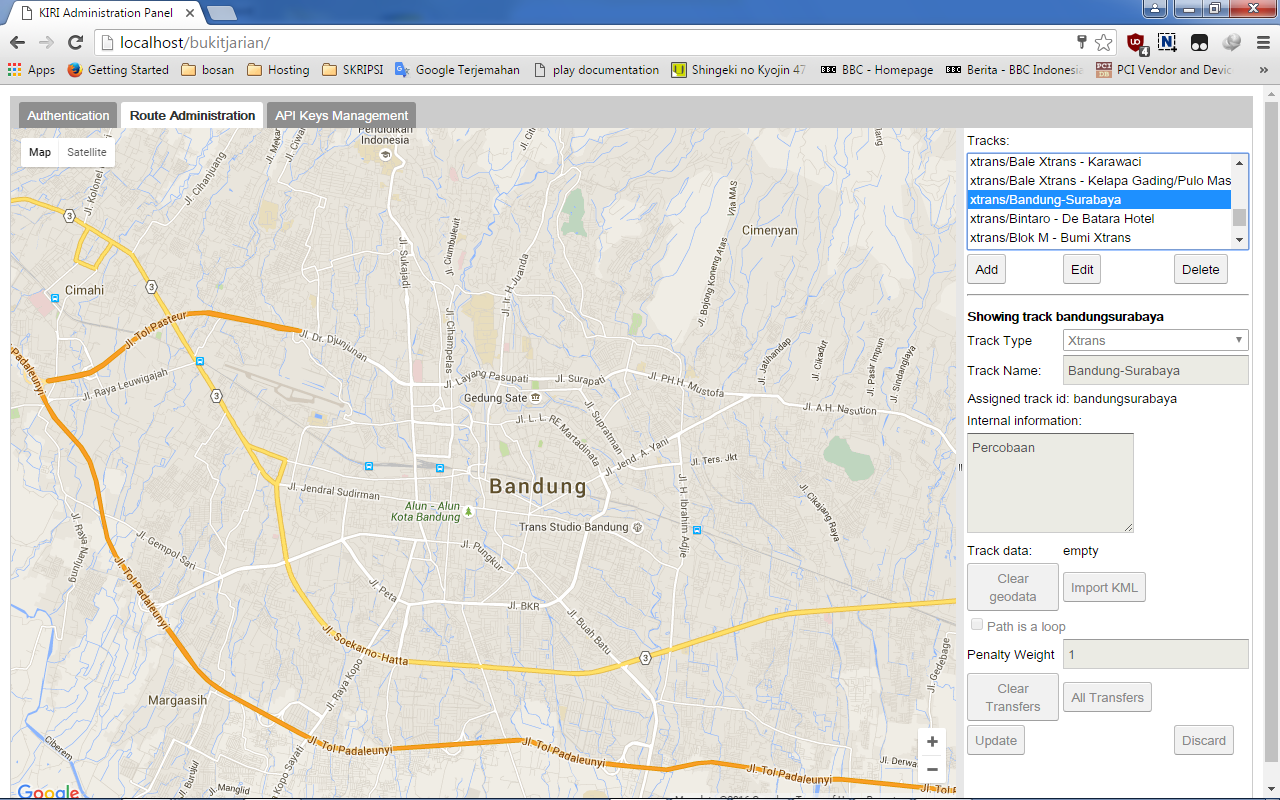
\includegraphics[scale=0.45]{Gambar/5_addtrack_2.png}
		\caption{Rute angkutan umum berhasil ditambahkan} 
		\label{fig:5_addtrack_2}
	\end{figure}

	\item \textbf{Bagian Mengubah Rute}\\
	Bagian ini merupakan bagian untuk mengubah data sebuah rute angkutan umum. Pengguna mengisi formulir untuk nama rute, informasi tambahan, bobot pengali rute, memilih jenis angkutan umum, dan memilih apakah terdapat \textit{loop} pada rute (Gambar \ref{fig:5_edittrack_1}). Jika formulir memenuhi persyaratan sistem, maka rute angkutan umum akan berubah (Gambar \ref{fig:5_edittrack_2}).

	\begin{figure}[htbp]
		\centering
			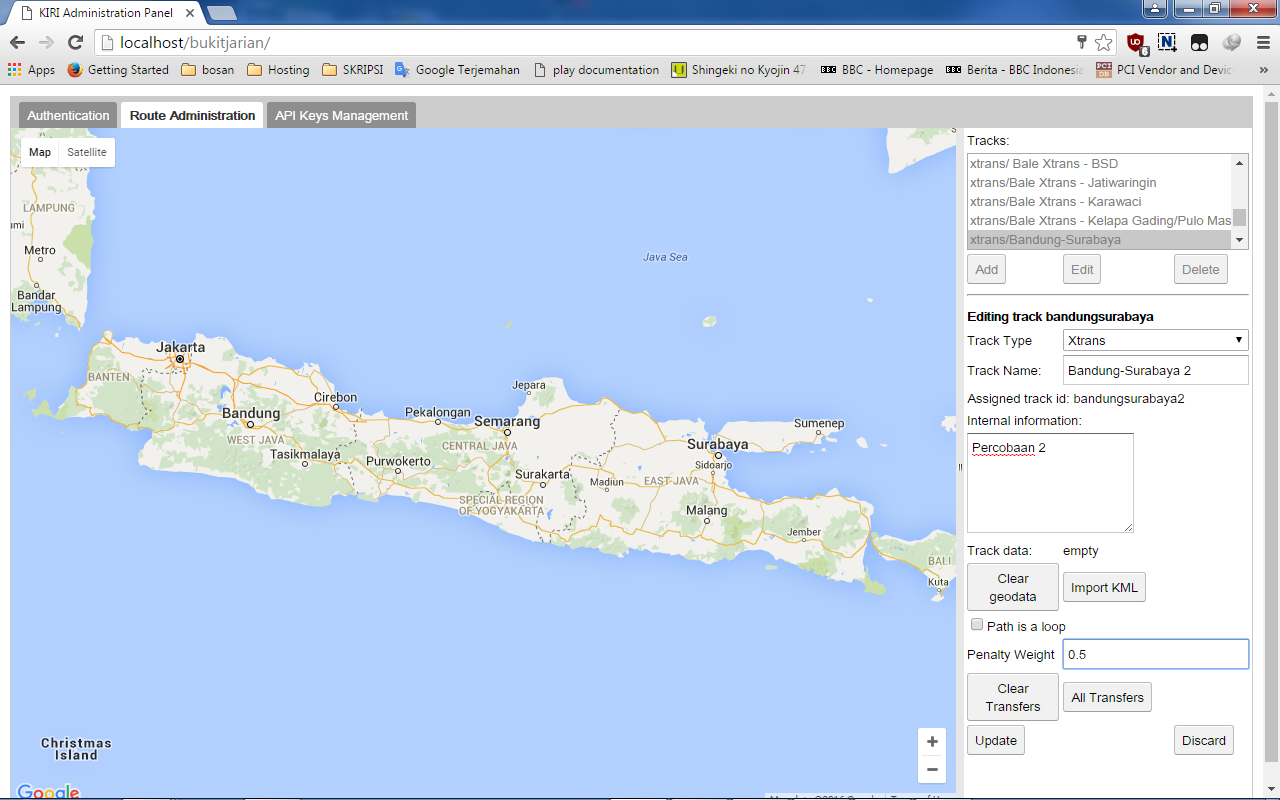
\includegraphics[scale=0.45]{Gambar/5_edittrack_1.png}
		\caption{Formulir mengubah data rute angkutan umum} 
		\label{fig:5_edittrack_1}
	\end{figure}

	\begin{figure}[htbp]
		\centering
			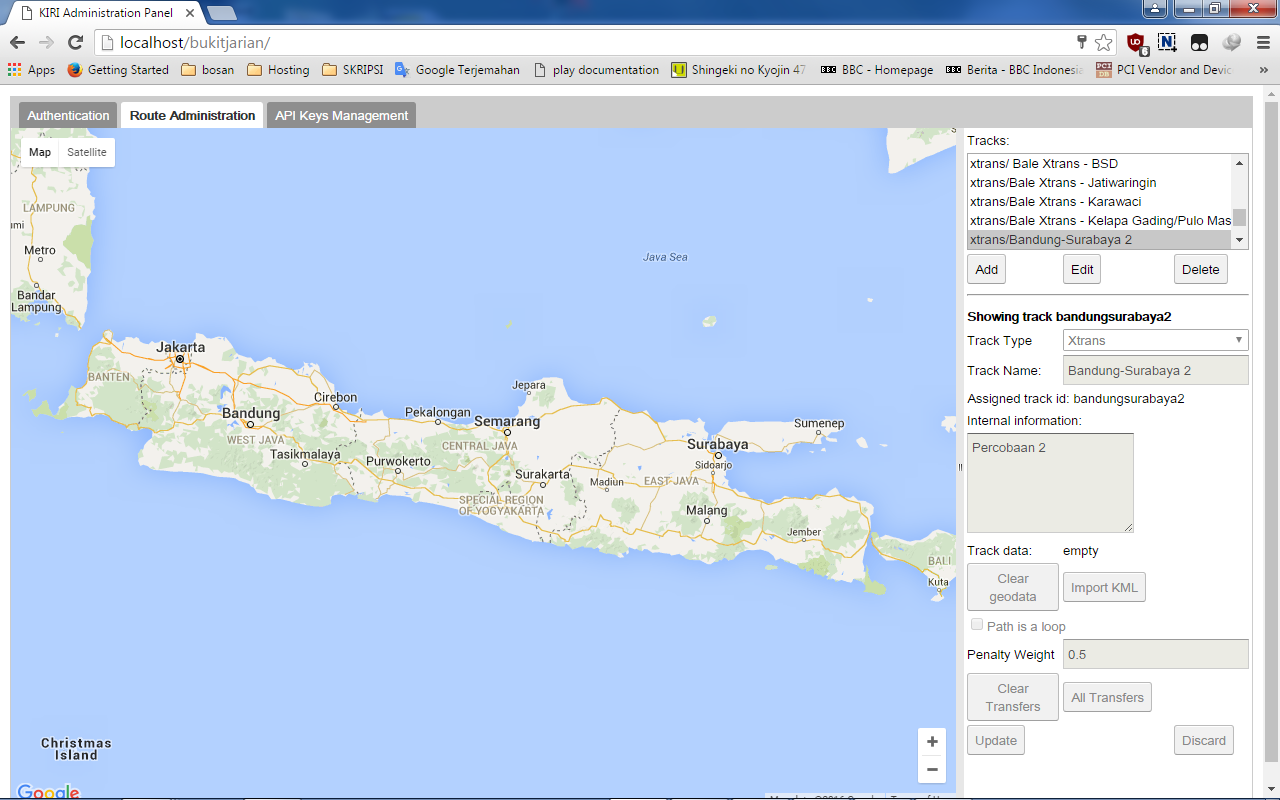
\includegraphics[scale=0.45]{Gambar/5_edittrack_2.png}
		\caption{Rute angkutan umum berhasil diubah} 
		\label{fig:5_edittrack_2}
	\end{figure}

	\item \textbf{Bagian Impor Data KML}\\
	Bagian ini merupakan bagian untuk menambahkan data geografis ke sebuah rute angkutan umum. Pengguna melakukan \textit{upload file} dalam format KML (Gambar \ref{fig:5_imporkml_1}). Jika \textit{file} memenuhi persyaratan sistem, maka akan muncul pesan keberhasilan dan peta akan berubah mengikuti data geografis pada \textit{file} tersebut (Gambar \ref{fig:5_imporkml_2}).

	\begin{figure}[htbp]
		\centering
			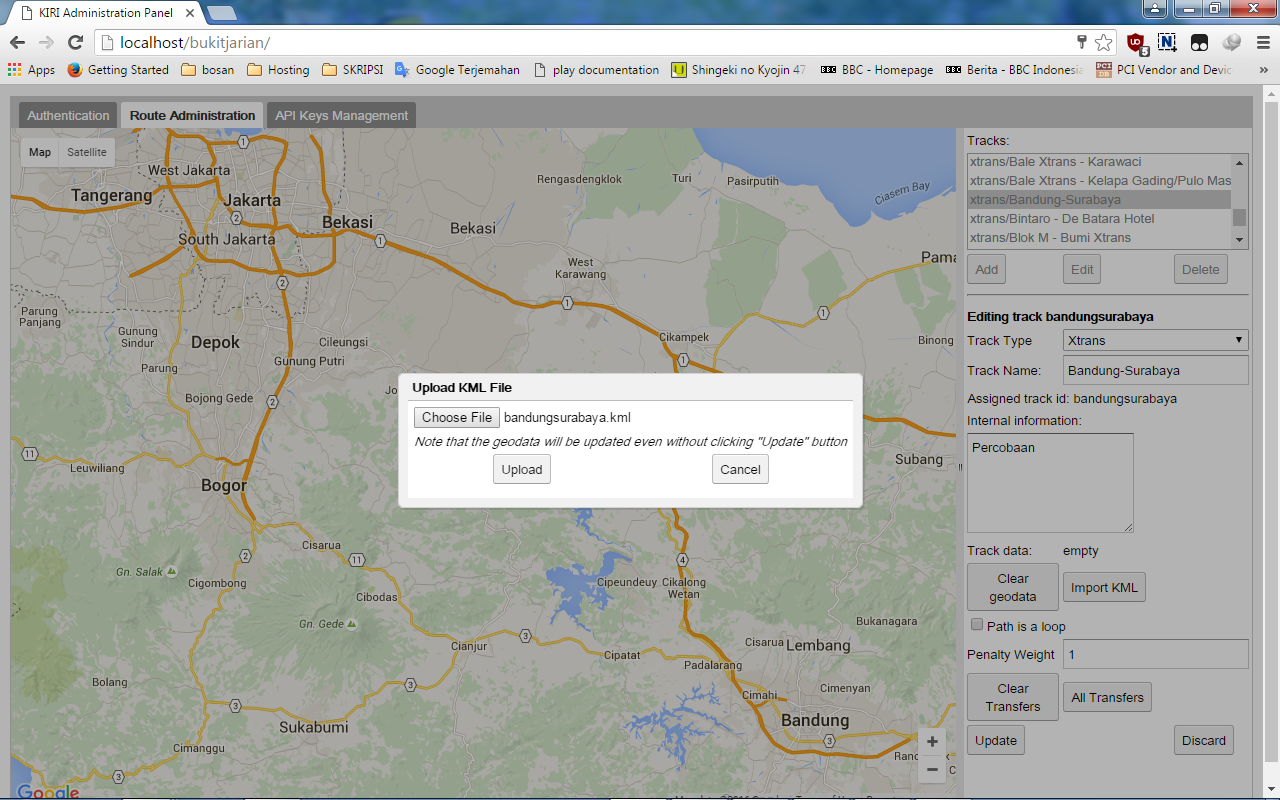
\includegraphics[scale=0.45]{Gambar/5_imporkml_1.png}
		\caption{\textit{Upload file} dalam format KML} 
		\label{fig:5_imporkml_1}
	\end{figure}

	\begin{figure}[htbp]
		\centering
			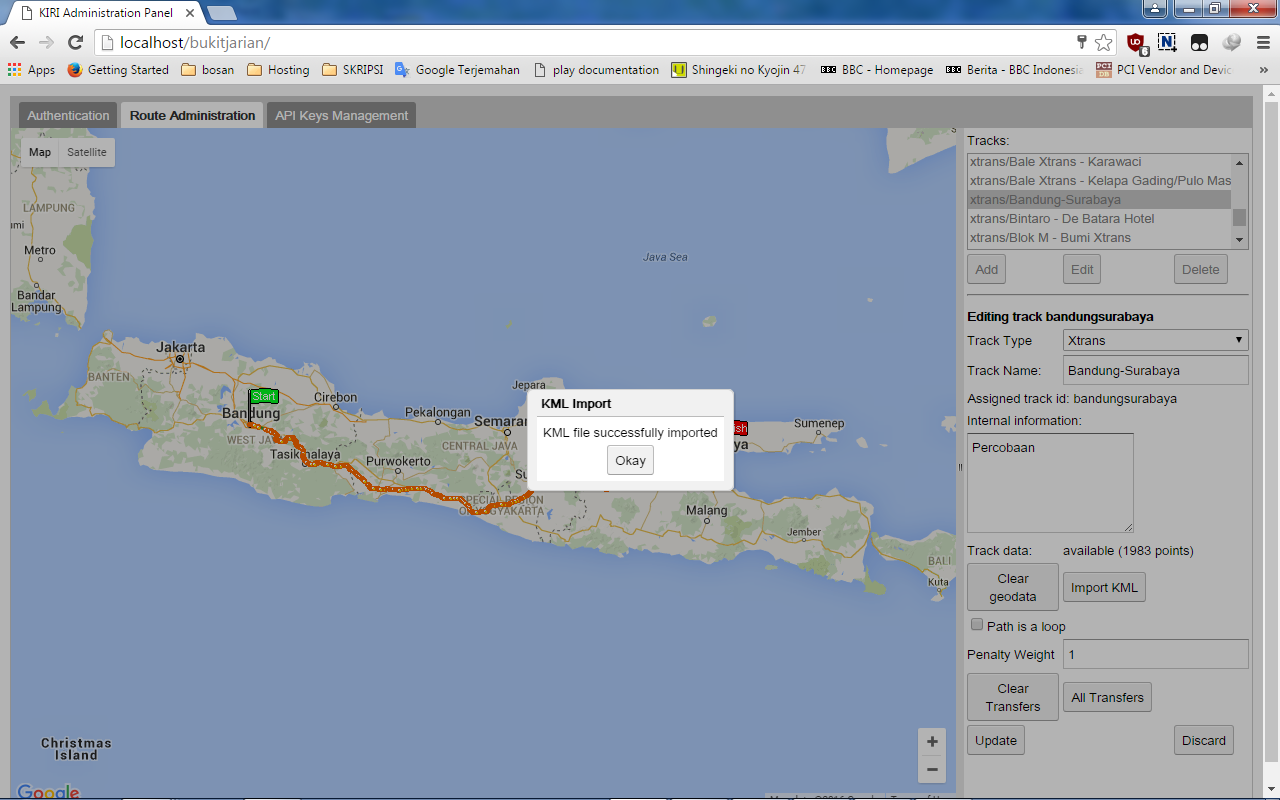
\includegraphics[scale=0.45]{Gambar/5_imporkml_2.png}
		\caption{Peta mengikuti data geografis \textit{file} yang di \textit{upload}} 
		\label{fig:5_imporkml_2}
	\end{figure}

	\item \textbf{Bagian Menghapus Data Geografis suatu Rute}\\
	Bagian ini merupakan bagian untuk menghapus data geografis sebuah rute angkutan umum. Pengguna melakukan verifikasi untuk menghapus data geografis suatu rute (Gambar \ref{fig:5_cleargeodata_1}). Data geografis pada peta terhapus (Gambar \ref{fig:5_cleargeodata_2}).

	\begin{figure}[htbp]
		\centering
			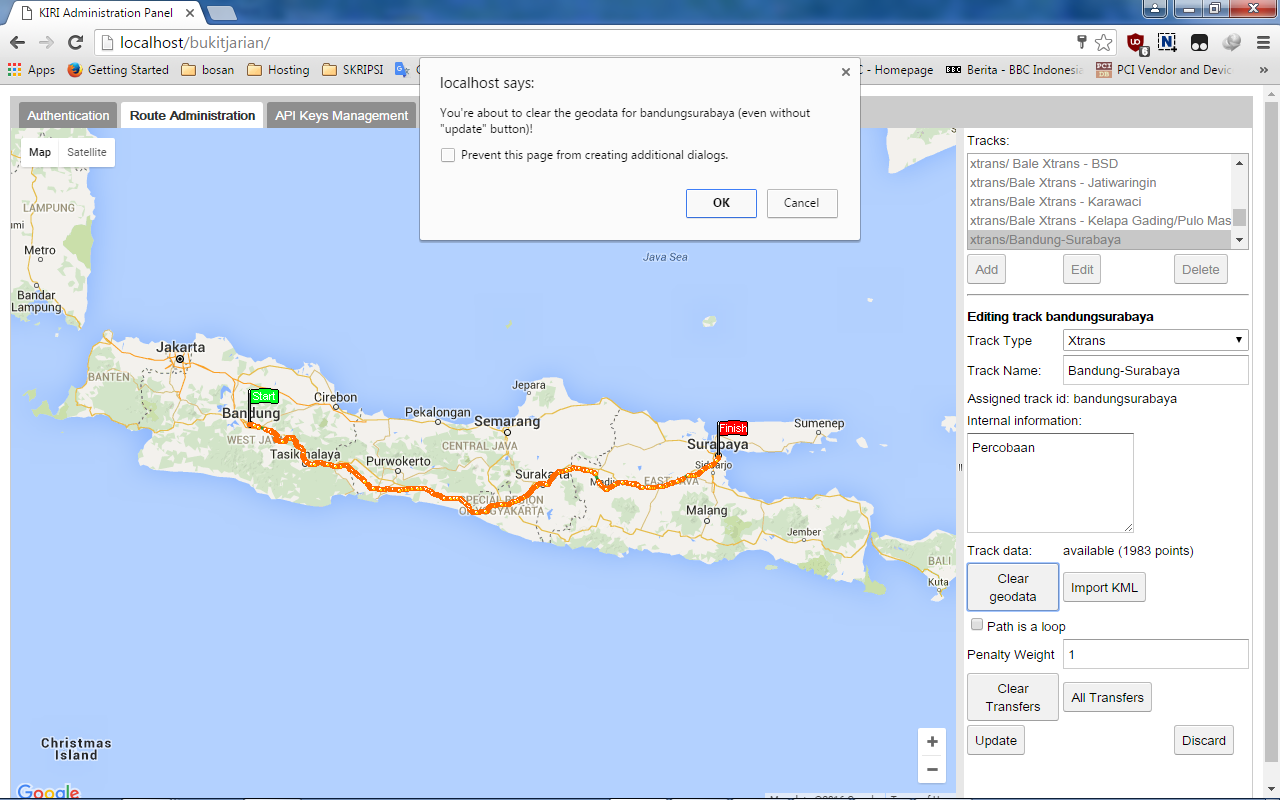
\includegraphics[scale=0.45]{Gambar/5_cleargeodata_1.png}
		\caption{Verifikasi penghapusan data geografis} 
		\label{fig:5_cleargeodata_1}
	\end{figure}

	\begin{figure}[htbp]
		\centering
			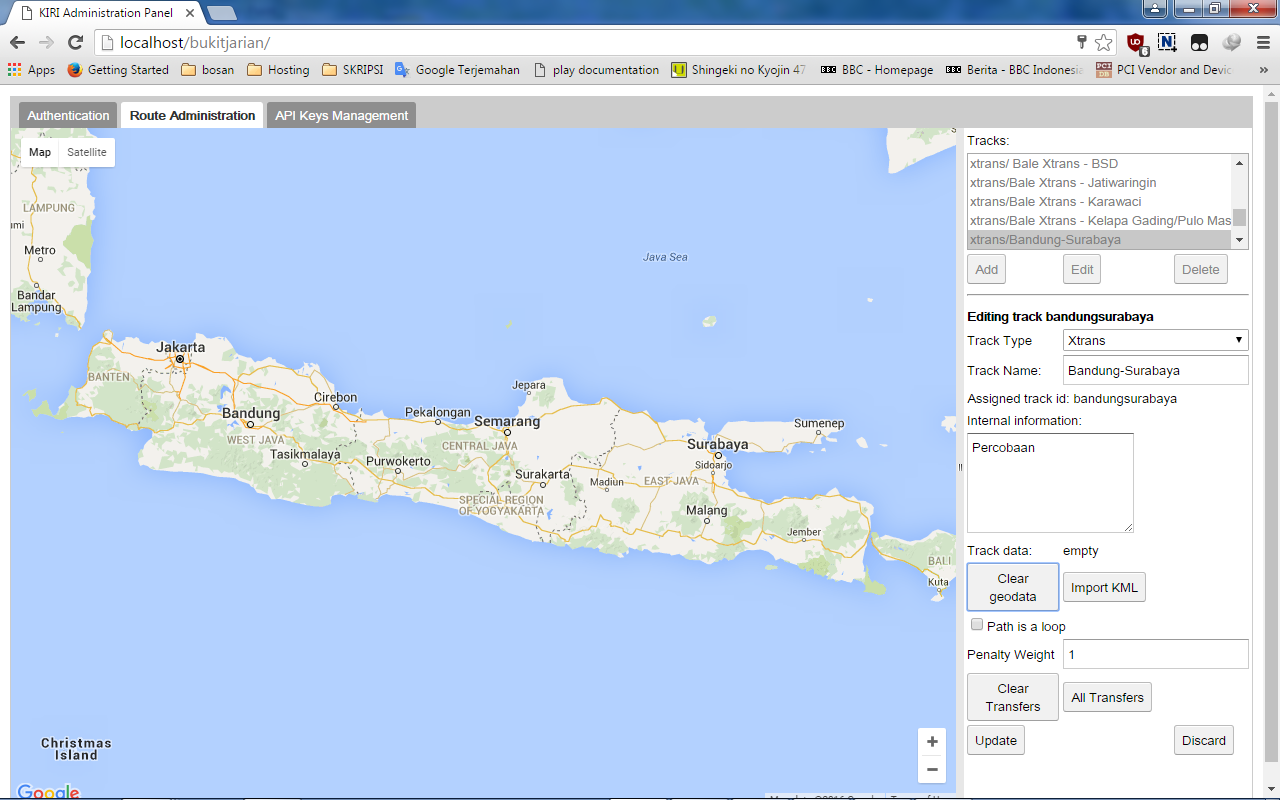
\includegraphics[scale=0.45]{Gambar/5_cleargeodata_2.png}
		\caption{Data geografis pada peta hilang} 
		\label{fig:5_cleargeodata_2}
	\end{figure}

	\item \textbf{Bagian Menghapus Rute}\\
	Bagian ini merupakan bagian untuk menghapus sebuah rute angkutan umum. Pengguna memilih dan melakukan verifikasi rute angkutan umum yang ingin dihapus (Gambar \ref{fig:5_deletetrack_1}). Rute angkutan umum terhapus dari sistem KIRI (Gambar \ref{fig:5_deletetrack_2}).

	\begin{figure}[htbp]
		\centering
			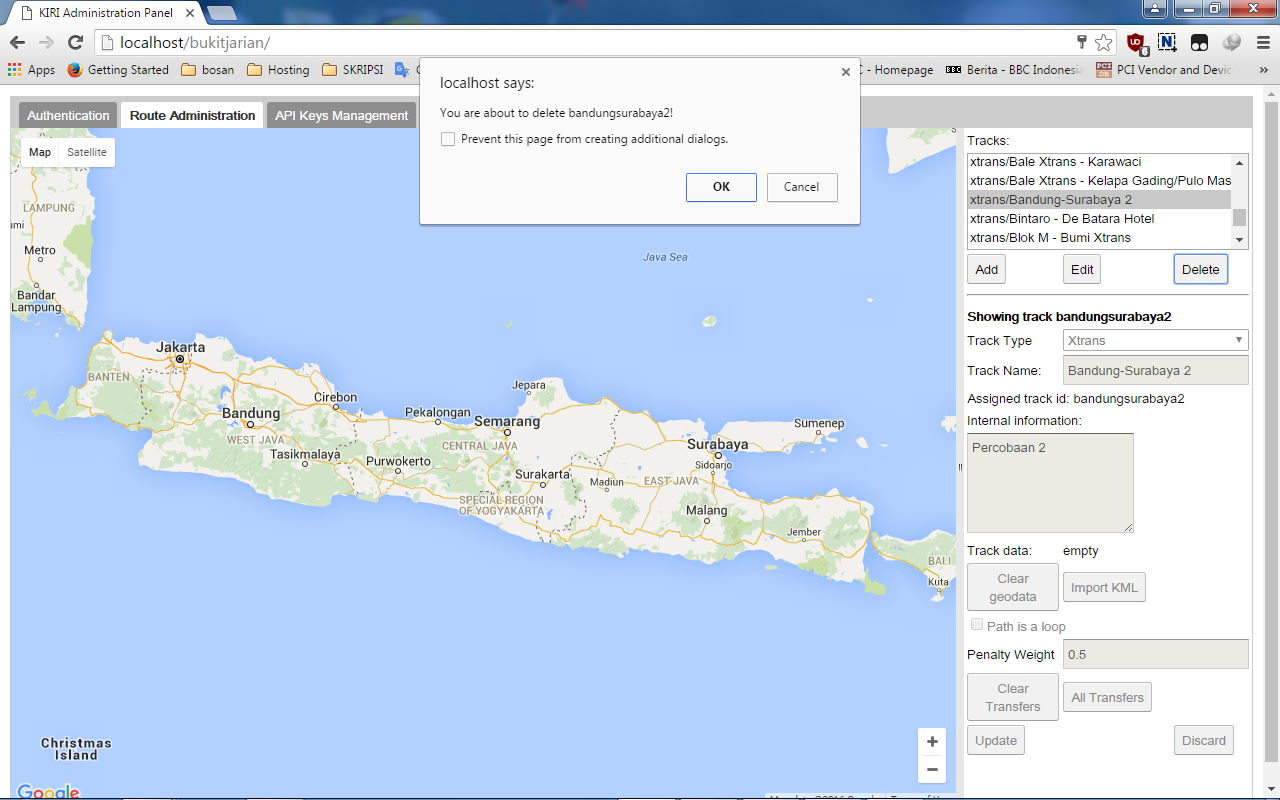
\includegraphics[scale=0.45]{Gambar/5_deletetrack_1.png}
		\caption{Memilih dan verifikasi penghapusan rute angkutan umum} 
		\label{fig:5_deletetrack_1}
	\end{figure}

	\begin{figure}[htbp]
		\centering
			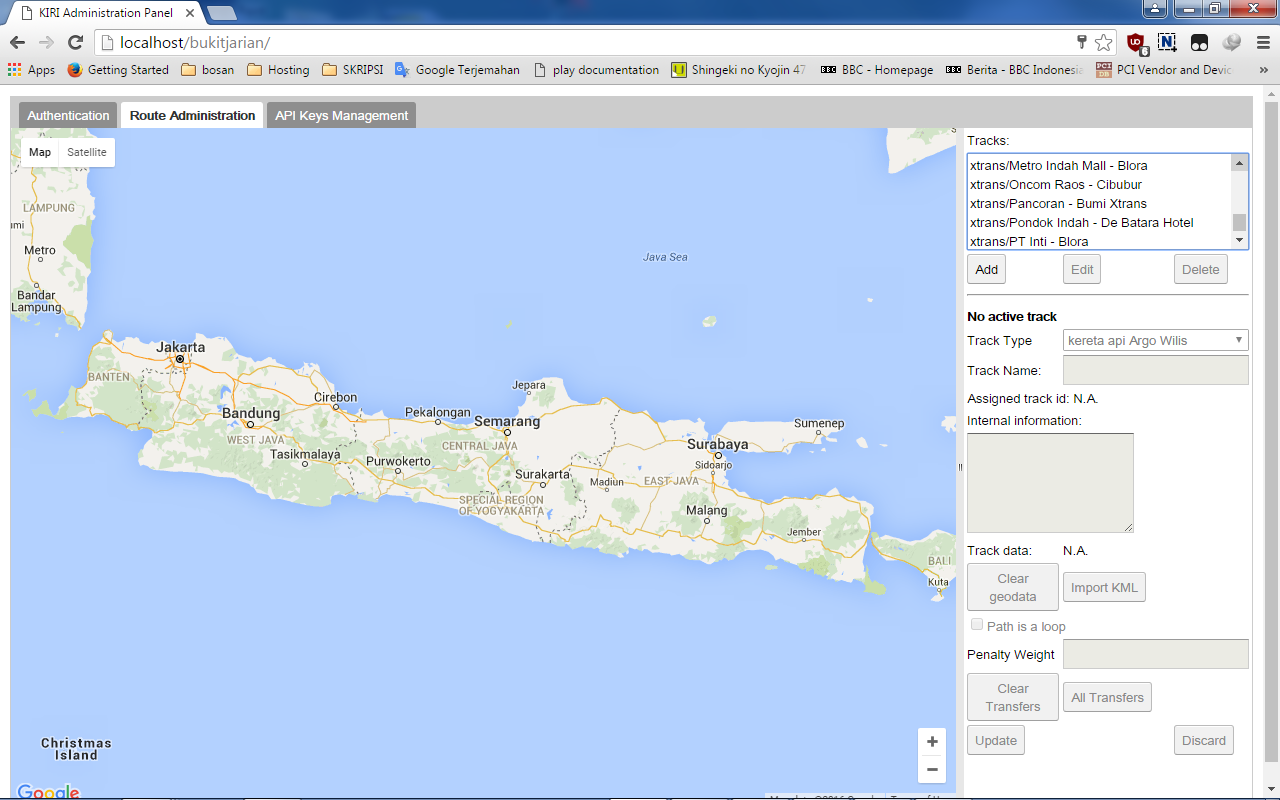
\includegraphics[scale=0.45]{Gambar/5_deletetrack_2.png}
		\caption{Rute angkutan umum hilang dari daftar} 
		\label{fig:5_deletetrack_2}
	\end{figure}

	\item \textbf{Bagian \textit{Logout}}\\
	Bagian ini merupakan bagian untuk keluar dari KIRI \textit{Dashboard}, yaitu kembali ke halaman \textit{login} (Gambar \ref{fig:5_logout}). 

	\begin{figure}[htbp]
		\centering
			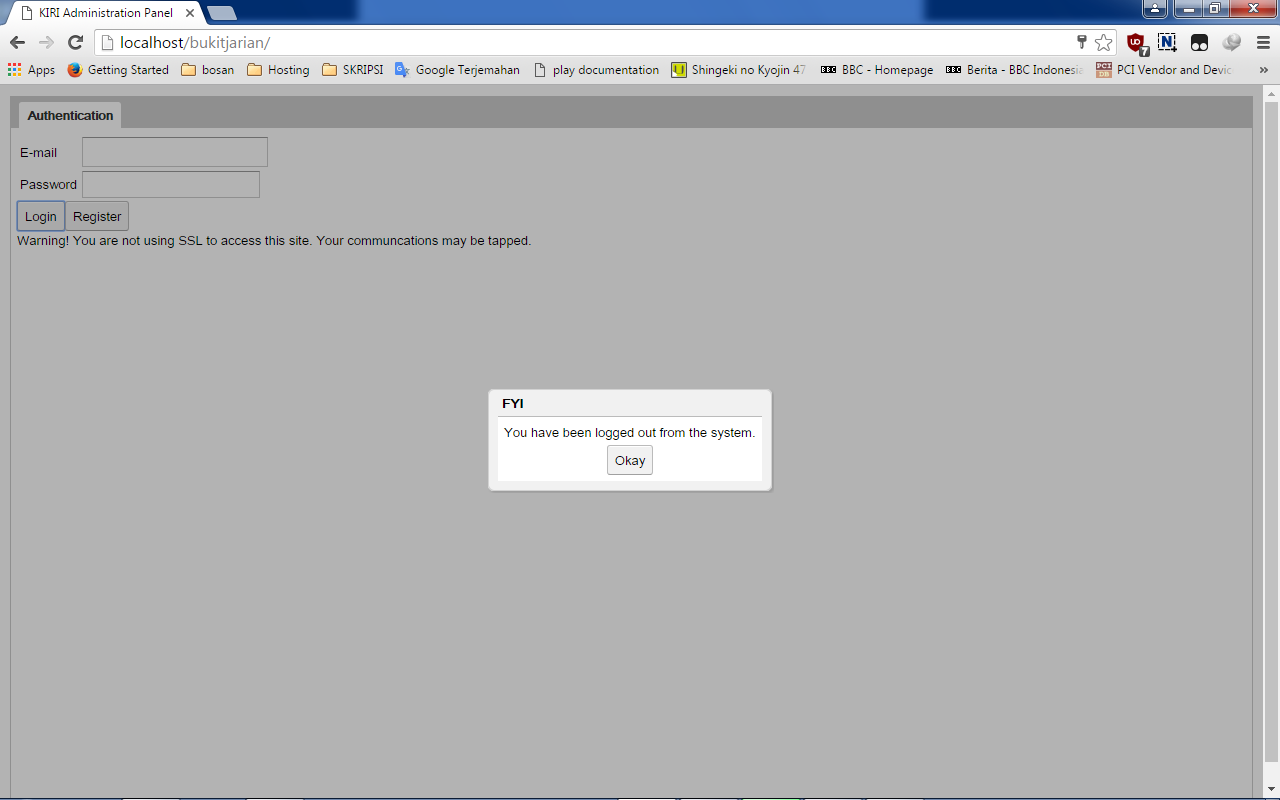
\includegraphics[scale=0.45]{Gambar/5_logout.png}
		\caption{\textit{Logout}} 
		\label{fig:5_logout}
	\end{figure}
\end{enumerate}

\section{Hasil Pengujian}
\label{sec:hasilpengujian}

\subsection{Pengujian Fungsional}
\label{sec:pengujianfungsional}
Pengujian fungsional dilakukan untuk mengetahui apakah sistem usulan sudah dapat menjalankan seluruh fungsi yang dimiliki oleh sistem kini. Pengujian ini dilakukan pada sistem operasi Windows. Pengujian ini dilakukan terhadap 16 bagian sistem usulan, detail hasilnya dapat dilihat pada Tabel \ref{table:hasilfungsional}.

\begin{table}[H]
	\centering
	\caption{Tabel Pengujian Fungsional}
		\begin{tabular}{|p{0.37cm}| p{3.5cm}| p{7cm}| p{2.5cm}|} \hline
		No & Aksi Pengguna	& Reaksi yang Diharapkan & Reaksi Sistem Usulan \\ \hline
		1. & Pengguna menjalankan aplikasi & Halaman \textit{login} ditampilkan & sesuai \\ \hline
		2. & Pengguna melakukan \textit{register} & Pengguna mendapatkan \textit{email} berupa sandi acak & sesuai \\ \hline
		3. & Pengguna melakukan \textit{login} & Pengguna masuk ke sistem KIRI \textit{Dashboard} & sesuai	\\ \hline
		4. & Pengguna melihat data pribadi & Sistem menampilkan data pribadi berupa alamat \textit{email}, nama lengkap, dan nama perusahaan milik pengguna & sesuai \\ \hline
		5. & Pengguna mengubah data pribadi & Sistem menampilkan pesan tanda keberhasilan mengubah data pribadi & sesuai\\ \hline
		6. & Pengguna melihat daftar API \textit{keys} & Sistem menampilkan daftar API \textit{keys} milik pengguna & sesuai \\ \hline
		7. & Pengguna menambahkan sebuah API \textit{key} & API \textit{key} baru muncul dalam daftar API \textit{keys} milik pengguna & sesuai \\ \hline
		8. & Pengguna mengubah data sebuah API \textit{key} & API \textit{key} yang dipilih pengguna berubah datanya sesuai dengan data yang dikirimkan pengguna & sesuai \\ \hline
		9. & Pengguna melihat daftar rute & Sistem menampilkan daftar rute angkutan umum milik sistem & sesuai \\ \hline
		10. & Pengguna melihat informasi rute secara detail & Sistem menampilkan informasi berupa tipe angkutan umum, nama rute, informasi tambahan (jika ada), data geografis dalam bentuk peta (jika ada), informasi \textit{loop}, dan bobot pengali & sesuai \\ \hline
		11. & Pengguna menambahkan rute & Rute baru muncul dalam daftar rute sistem & sesuai \\ \hline
		12. & Pengguna mengubah data sebuah rute & Data rute berubah sesuai dengan data yang dikirimkan oleh pengguna & sesuai  \\ \hline
		13. & Pengguna melakukan impor data KML & Tampilan peta berubah mengikuti data geografis yang dikirimkan pengguna & sesuai \\ \hline
		14. & Pengguna menghapus data geografis suatu rute & Data geografis yang terdapat pada peta terhapus & sesuai \\ \hline
		15. & Pengguna menghapus sebuah rute & Rute angkutan umum yang dipilih pengguna terhapus dari daftar rute sistem & sesuai  \\ \hline
		16. & Pengguna melakukan \textit{logout} & tampilan sistem berubah kembali seperti semula (halaman \textit{login}) & sesuai  \\ \hline
		\end{tabular}
	\label{table:hasilfungsional}
\end{table}

\subsection{Pengujian Eksperimental}
\label{sec:pengujianeksperimental}
Pengujian eksperimental yang dilakukan adalah pengujian terhadap waktu eksekusi. Pengujian dilakukan dengan membandingkan sistem kini dan sistem usulan. Pengujian dilakukan terhadap 16 bagian sistem dimana setiap bagian diuji sebanyak 5 kali percobaan, detail hasil pengujian dapat dilihat pada Tabel \ref{table:hasileksperimental1}, Tabel \ref{table:hasileksperimental2}, Gambar \ref{fig:5_pengujianwaktu_1}, dan Gambar \ref{fig:5_pengujianwaktu_2}.

\begin{table}[H]
	\centering
	\caption{Tabel Pengujian Eksperimental Sistem Kini (dalam mili sekon)}
		\begin{tabular}{|p{0.37cm}| p{7cm}| p{1cm}| p{1cm}| p{1cm}| p{1cm}| p{1cm}| p{1cm}|} \hline
		No & Aksi & 1 & 2 & 3 & 4 & 5 & rata-rata \\ \hline
		1. & Menjalankan aplikasi (halaman \textit{login}) & 1298	&	1382	&	1312	&	1308	&	1322	&	1324.4 \\ \hline
 		2. & \textit{Register} & 5082	&	4387	&	4607	&	4963	&	4352	&	4678.2 \\ \hline
		3. & \textit{Login} & 176	&	178	&	198	&	186	&	181	&	183.8 \\ \hline
		4. & Melihat data pribadi pengguna & 30	&	32	&	33	&	34	&	36	&	33 \\ \hline
		5. & Mengubah data pribadi pengguna & 90	&	127	&	139	&	139	&	147	&	128.4 \\ \hline
		6. & Melihat daftar API \textit{keys} & 35	&	34	&	37	&	30	&	29	&	33 \\ \hline
		7. & Menambahkan API \textit{key} & 138	&	137	&	141	&	139	&	145	&	140 \\ \hline
		8. & Mengubah API \textit{key} & 61	&	51	&	57	&	63	&	59	&	58.2 \\ \hline
		9. & Melihat daftar rute & 30	&	37	&	32	&	37	&	27	&	32.6 \\ \hline
		10. & Melihat informasi rute secara detail & 42	&	41	&	38	&	39	&	45	&	41 \\ \hline
		11. & Menambahkan rute & 154	&	157	&	159	&	151	&	151	&	154.4 \\ \hline
		12. & Mengubah rute & 145	&	161	&	146	&	144	&	155	&	150.2 \\ \hline
		13. & Impor data KML & 229	&	257	&	246	&	232	&	245	&	241.8 \\ \hline
		14. & Menghapus data geografis suatu rute & 150	&	146	&	155	&	114	&	151	&	143.2 \\ \hline
		15. & Menghapus rute & 198	&	192	&	154	&	184	&	177	&	181 \\ \hline
		16. & \textit{Logout} & 90	&	82	&	83	&	91	&	77	&	84.6 \\ \hline
		\end{tabular}
	\label{table:hasileksperimental1}
\end{table}

\begin{table}[H]
	\centering
	\caption{Tabel Pengujian Eksperimental Sistem Usulan (dalam mili sekon)}
		\begin{tabular}{|p{0.37cm}| p{7cm}| p{1cm}| p{1cm}| p{1cm}| p{1cm}| p{1cm}| p{1cm}|} \hline
		No & Aksi & 1 & 2 & 3 & 4 & 5 & rata-rata \\ \hline
		1. & Menjalankan aplikasi (halaman \textit{login}) & 1170	&	1220	&	1180	&	1210	&	1212	&	1198.4 \\ \hline
 		2. & \textit{Register} & 9072	&	9280	&	9281	&	9174	&	9088	&	9179 \\ \hline
		3. & \textit{Login} & 198	&	192	&	190	&	195	&	193	&	193.6 \\ \hline
		4. & Melihat data pribadi pengguna & 30	&	26	&	35	&	23	&	26	&	28 \\ \hline
		5. & Mengubah data pribadi pengguna & 230	&	234	&	217	&	222	&	224	&	225.4 \\ \hline
		6. & Melihat daftar API \textit{keys} & 21	&	20	&	22	&	27	&	28	&	23.6 \\ \hline
		7. & Menambahkan API \textit{key} & 53	&	63	&	61	&	66	&	63	&	61.2 \\ \hline
		8. & Mengubah API \textit{key} & 58	&	53	&	56	&	58	&	53	&	55.6 \\ \hline
		9. & Melihat daftar rute & 26	&	30	&	30	&	16	&	25	&	25.4 \\ \hline
		10. & Melihat informasi rute secara detail & 33	&	27	&	43	&	44	&	46	&	38.6 \\ \hline
		11. & Menambahkan rute & 131	&	144	&	138	&	105	&	136	&	130.8 \\ \hline
		12. & Mengubah rute & 122	&	133	&	144	&	118	&	135	&	130.4 \\ \hline
		13. & Impor data KML & 244	&	213	&	250	&	168	&	234	&	221.8 \\ \hline
		14. & Menghapus data geografis suatu rute & 126	&	94	&	81	&	123	&	70	&	98.8 \\ \hline
		15. & Menghapus rute & 159	&	162	&	164	&	162	&	172	&	163.8 \\ \hline
		16. & \textit{Logout} & 74	&	69	&	78	&	68	&	75	&	72.8 \\ \hline
		\end{tabular}
	\label{table:hasileksperimental2}
\end{table}

% \begin{table}[H]
% 	\centering
% 	\caption{Tabel Perbandingan Sistem Kini dan Sistem Usulan (dalam mili sekon)}
% 		\begin{tabular}{|p{0.37cm}| p{7cm}| p{2.4cm}| p{2.4cm}|} \hline
% 		No & Aksi & Sistem Kini & Sistem Usulan \\ \hline
% 		1. & Menjalankan aplikasi (halaman \textit{login}) & 1324.4 & 1198.4\\ \hline
%  		2. & \textit{Register} & 4678.2 & 9179\\ \hline
% 		3. & \textit{Login} & 183.8 & 193.6\\ \hline
% 		4. & Melihat data pribadi pengguna & 33 & 28\\ \hline
% 		5. & Mengubah data pribadi pengguna & 128.4 & 225.4\\ \hline
% 		6. & Melihat daftar API \textit{keys} & 33 & 23.6\\ \hline
% 		7. & Menambahkan API \textit{key}& 140  & 61.2\\ \hline
% 		8. & Mengubah API \textit{key} & 58.2 & 55.6\\ \hline
% 		9. & Melihat daftar rute & 32.6 & 25.4\\ \hline
% 		10. & Melihat informasi rute secara detail & 41 & 38.6\\ \hline
% 		11. & Menambahkan rute 	& 154.4 & 130.8\\ \hline
% 		12. & Mengubah rute & 150.2 & 130.4\\ \hline
% 		13. & Impor data KML 	& 241.8 & 221.8\\ \hline
% 		14. & Menghapus data geografis suatu rute 	& 143.2 & 98.8\\ \hline
% 		15. & Menghapus rute & 181 & 163.8\\ \hline
% 		16. & \textit{Logout} & 84.6 & 72.8\\ \hline
% 		\end{tabular}
% 	\label{table:hasileksperimental3}
% \end{table}

\begin{figure}[htbp]
	\centering
		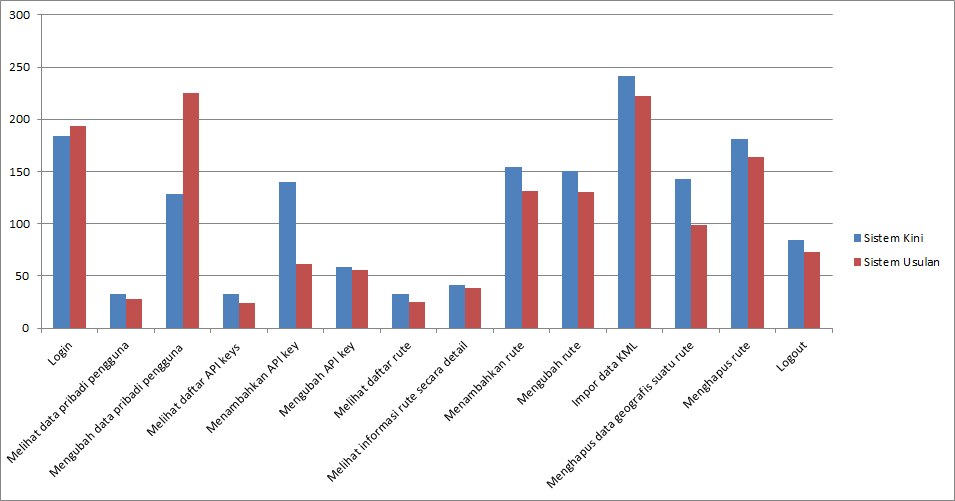
\includegraphics[scale=0.6]{Gambar/5_pengujianwaktu_1.png}
	\caption{Grafik rata-rata waktu eksekusi 1 (dalam mili sekon)} 
	\label{fig:5_pengujianwaktu_1}
\end{figure}

\begin{figure}[htbp]
	\centering
		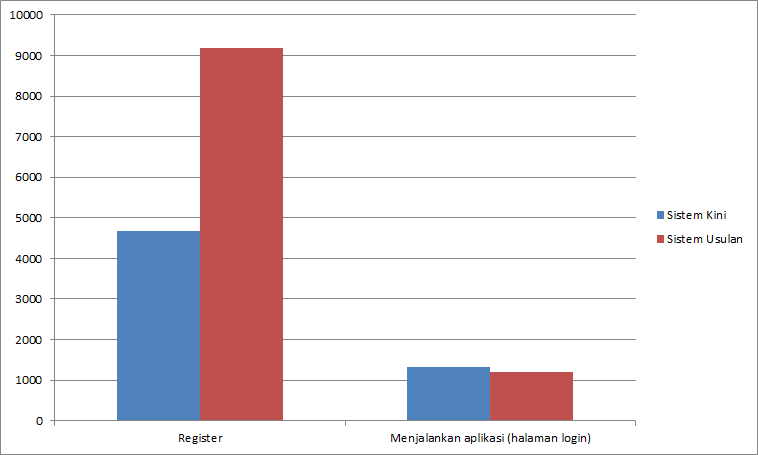
\includegraphics[scale=0.7]{Gambar/5_pengujianwaktu_2.png}
	\caption{Grafik rata-rata waktu eksekusi 2 (dalam mili sekon)} 
	\label{fig:5_pengujianwaktu_2}
\end{figure}

Berdasarkan hasil pengamatan terhadap Gambar \ref{fig:5_pengujianwaktu_1} dan Gambar \ref{fig:5_pengujianwaktu_2}, didapatkan informasi bahwa seluruh bagian sistem usulan memiliki waktu eksekusi lebih cepat dibandingkan dengan sistem kini, kecuali pada bagian \textit{register}, \textit{login}, dan mengubah data pribadi pengguna. Dikarenakan terdapat perbedaan hasil pada 3 bagian, yaitu: bagian \textit{register}, \textit{login}, dan mengubah data pribadi pengguna, maka peneliti melakukan analisis terhadap kode sistem kini dan sistem usulan pada 3 bagian tersebut. Berikut adalah hasil analisis terhadap 3 bagian tersebut:
\begin{enumerate}
	\item \textit{Login} dan mengubah data pribadi pengguna\\
	Pada bagian \textit{login} dan mengubah data pribadi pengguna menggunakan algoritma bcrypt dalam melakukan \textit{hashing} terhadap sandi. Pada algoritma bcrypt, terdapat sebuah nilai (berupa angka) untuk menentukan tingkat kompleksitas proses \textit{hashing}\cite{jbcrypt}. Semakin tinggi angka yang diberikan maka kompleksitas proses \textit{hashing} semakin tinggi dan hasilnya juga semakin sulit untuk diretas. Pada sistem kini ditemukan bahwa nilai yang diberikan adalah 8 (baris 54 dan 370 Kode \ref{lst:handle.php}) dan pada sistem usulan adalah 10\cite{jbcrypt}. Oleh karena itu, peneliti menduga bahwa perbedaan nilai tersebut adalah penyebab bagian \textit{login} dan mengubah data pribadi pengguna pada sistem usulan menjadi lebih lambat dibandingkan bagian sistem kini (kompleksitas proses \textit{hashing} sistem usulan lebih tinggi).
	\item \textit{Register}\\
	Berdasarkan analisis terhadap kode sistem usulan, peneliti mendapatkan informasi bahwa struktur kode bagian ini umumnya sama dengan struktur kode bagian lainnya, kecuali struktur kode pada metode pengiriman \textit{email}. Pada sistem kini pengiriman \textit{email} dilakukan dengan menggunakan PHPMailer (baris 317 Kode \ref{lst:utils.php}) dan pada sistem usulan pengiriman \textit{email} dilakukan dengan menggunakan JavaMail API (baris 114 Kode \ref{lst:authenticationmanager.java}).  Peneliti menduga terdapat perbedaan protokol internet dalam pengiriman \textit{email} pada PHPMailer dan JavaMail API yang menyebabkan perbedaan waktu yang cukup lama (4500.8 mili sekon). 
\end{enumerate}

